\documentclass[a4paper]{article}
\usepackage{amsmath}
\usepackage{amssymb}
\usepackage{fancyhdr}
\usepackage{a4wide}
\usepackage{geometry}
\usepackage[utf8]{inputenc}
\usepackage{graphicx}
\geometry{a4paper,left=2cm,right=2cm, top=3cm, bottom=3cm}
\usepackage{listings}
\lstset{language=xml}
\newcommand{\oh}[1]{$\mathcal{O}(#1)$}
\newcommand{\titel}[1]{\fancyhead[C]{#1}}
\newcommand{\name}{\fancyhead[L]{Alexander Landmesser}}
\newcommand{\matrikel}{\fancyhead[R]{}}
\newcommand{\pl}{\hspace*{1cm}}
\begin{document}
\title{Ausgewählte Kapitel ADS}
\maketitle
\section{Datenstrukturen für Mengen}
\subsection{Union-Find-Problem}
Verwaltung von diskunkten Mengen\\
%TODO BILD 1: Mengen Beispiel
\subsubsection*{Problem}
Verwalte eine Partition (Zerlegung in disjunkte Teilmengen) der Menge \{1,...,n\} unter folgenden Operationen.\\
Jede Teilmenge (Block) besitzt einen eindeutigen Namen aus \{1,..,n\}.
\begin{itemize}
\item FIND(x): $x\in \{1,..,n\}$ Liefert den Namen der Teilmenge, die x enthält
\item UNION(A,B,C): Vereinigt die Teilmengen mit Namen A und B zu einer Teilmenge mit dem Namen C.
\end{itemize}
\subsubsection*{Initialisierung}
Wir starten mit der Partitionierung: $\{\{1\},..,\{n\}\}$ mit dem Namen $i$ für $\{i\}$,$1\leq i \leq n$\\
Analyse: Kosten für 1 Union (worst case)\\
Amortisiert: Kosten für $n-1$ mögliche UNIONs\\
$\rightarrow$ Kosten von $n-1$ UNIONs und m FINDs\\
\subsubsection*{Lösungen}
\underline{\textbf{1. Lösung} (einfach)}\\
Verwende ein Feld name[1..n] mit name[x] = Name des Blocks der x enthält. $1\leq x \leq n$\\
\begin{lstlisting}
for i=1 to n do
	name[i] <- i
od
\end{lstlisting}
FIND(x): return name[x] : \oh{n}\\
UNION(A,B,C): \oh{n}
\begin{lstlisting}
for i=1 to n do
	if name[i] = A OR name[i] = B
	then name[i] <- C
	fi
od
\end{lstlisting}
Gesamtlaufzeit (Lemma 1):\\
$n-1$ UNIONs und m FINDs kosten \oh{n^2+m}\\
\underline{\textbf{2. Lösung} (Verbesserung)}\\
1. Find unverändert\\
2. Ändere den Namen der kleineren Menge in den Namen der größeren (Relabel the smaller half)\\
Zusätzliche Felder:
\begin{itemize}
\item size[1..n]: size[A] = Anzahl Elemente im Block A, initialisiert mit 1
\item L[1..n]: L[A] = Liste aller Elemente in Block A, initialisiert L[i] = \{i\}
\end{itemize}
FIND(x) bleibt gleich\\
UNION(A,B):
\begin{lstlisting}[escapechar=!]
if size[A] !$\leq$! size[B]
then
	forall i in L[A] do
		name[i]!$\leftarrow$! B
	od
	size[B] += size[A]
	L[B] !$\leftarrow$! L[B] concatenate L[C]
else
	symmetrisch
\end{lstlisting}
Die Menge heißt jetzt A oder B\\
Effekt: UNION(A,B,..) hat Laufzeit \oh{min(|A|,|B|)}\\
Worst Case eines UNION dieser Folge von UNIONs: \oh{\frac{n}{2}} = \oh{n} (kann nur einmal vorkommen)\\
Wie oft kann sich name[x] für ein bestimmtes $x:1\leq x\leq n$ ändern?\\
Beobachtung:
\begin{itemize}
\item Am Anfang ist jedes Element x in einer ein-elementigen Menge
\item Am Ende sind alle Elemente in einer Menge der Größe n
\item Immer wenn ein Element x seinen Namen ändert befindet es sich danach in einer doppelt so großen Menge (nach dem UNION)
\end{itemize}
$\Rightarrow$ Jedes Element $x\in \{1,..,\}$ kann maximal $log(n)$ mal seinen Namen ändern.\\
\underline{Satz 1:}
Bei UNION-FIND mit "Relabel the smaller half" sind die Gesamtkosten einer beliebigen Folge von n-1 UNIONS und m Finds \oh{m+n*log(n)}\\
Im Schnitt (amortisiert) kostet ein UNION $log(n)$\\
\underline{\textbf{3. Lösung}}\\
Lösung 1 und 2 haben FIND effizient gelöst, hier UNION\\
Jeder Block wird als Baum dargestellt. Die Knoten repräsentieren die Elemente des Blocks. In der Wurzel steht der Name des Blocks.\\
%TODO BILD 2: Bäume der Mengen
UNION(A,B,E): Mache die Wurzel von A zum Kind der Wurzel von B und nenne die Wurzel um in E.\\
FIND(x): Starte bei Element (Knoten) x und laufe bis zur Wurzel, dort steht der Name $\rightarrow$ \oh{Tiefe\ von\ x}\\
\textbf{Realisierung der Datenstruktur durch Felder:}\\
$vater[i]=\left\lbrace \begin{array}{c}Vater\ von\ i\ in\ seinem\ Baum\\ 0,\ falls\ i\ Wurzel\end{array}\right.$\\ %HELP
$name[i]=$Name des Blocks mit Wurzel i (at nur Bedeutung, falls i Wurzel)\\
$wurzel[i]=$ Wurzel des Blocks mit Namen i\\
\begin{tabular}{ l |c| r }
Initialisierung: & FIND(x): & UNION(A,B,C):\\
\begin{lstlisting}
for i=1 to n do
	vater[i] = 0
	name[i] = i
	wurzel[i] = i
od
\end{lstlisting}
&
\begin{lstlisting}
while vater[x] != 0 do
	x = vater[x]
od
return name[x]
\end{lstlisting}&
\begin{lstlisting}
r1 = wurzel[A]
r2 = wurzel[B]
vater[r1] = r2
name[r2] = C
wurzel[C] = r2
\end{lstlisting}

\end{tabular}\\
Analyse:
\begin{itemize}
\item UNION: \oh{1} worst case
\item FIND(x): Tiefe von x (max Höhe des entstehenden Baums, n-1 möglich)
\end{itemize}
\underline{\textbf{4. Lösung (Weighted Union rule):}}\\
Vermeide große Tiefen, dafür hänge den kleineren Baum (Anzahl Knoten) an den größeren\\
Alternativ: Hänge den Baum mit kleinerer höhe an den tieferen.\\
Realisierung: Zusätzliches Feld\\
size[i] = Anzahl Knoten um Unterbaum mit Wurzel i\\
\begin{tabular}{ l |c |r }
Initialisierung: & FIND(x) (wie bei 3): & UNION(A,B,C):\\
\begin{lstlisting}
for i=1 to n do
	vater[i] = 0
	name[i] = i
	wurzel[i] = i
	size[i] = 1
od
\end{lstlisting}
&
\begin{lstlisting}[escapechar=|]
while vater[x] != 0 do
	x = vater[x]
od
return name[x]
\end{lstlisting}&
\begin{lstlisting}[escapechar=|]
r1 = wurzel[A]
r2 = wurzel[B]
if size[r1] |$\leq $| size[r2] then
	vater[r1] = r2
	name[r2] = C
	wurzel[C] = r2
	size[r2] += size[r1]
else
	symmetrisch
\end{lstlisting}
\end{tabular}
Zeige Laufzeit \oh{log(n)}:\\
Sei für jeden Knoten x die höhe(x) die Hohe von x in seinem Baum (maximale Pfad zu Blatt), Blatt=0\\
size(x): Anzahl der Knoten im Unterbaum mit Wurzel x (Gewicht)\\
\underline{Lemma}: Bei weighted Union rule gilt stets, dass $size(x)\geq 2^{\text{höhe}(x)}$ für alle Knoten x.\\
Beweis: Induktion über höhe(x):\\
\begin{lstlisting}[escapechar=!]
Vorasussetzung:
	h!ö!he(x) = 0: x ist Blatt -> size(x)=1=!$2^0$!
Anfang:
	size(y) !$\geq 2^{\text{höhe}(y)}$!
Schritt:
	Sei h!ö!he(x) > 0
	Sei y ein Kind von x mit h!ö!he(x)-1
	Betrachte die UNION Operation bei der x zum Vater von y wurde.
	Seien !$\overline{size}(x)$! und !$\overline{size}(y)$! die Gewichte vor der UNION Operaion, dann gilt:
	1) size(y) = !$\overline{size}(y)$!, da sich das Gewicht nur !für! Wurzeln !ä!ndern kann
	2) !$\overline{size}(x) \geq \overline{size}(y)$! durch weighted union rule
	3) Nach der Operation: !$size(x) \geq \overline{size}(x)+\overline{size}(y)$!
		!$\geq 2*\overline{size}(y)$! wegen 2.
		!$\geq 2*size(y)$! wegen 1.
		!$\geq 2*2^{\text{höhe}(y)}$! nach IA
		!$=2^{\text{höhe}(y)+1} = 2^{\text{höhe}(x)}$!
\end{lstlisting}
Da Anzahl der Knoten $n \Rightarrow size(x) \leq n$ gilt:\\
\hspace*{1cm}$\Rightarrow n\geq size(x)\geq 2^{hoehe(x)}$ für alle x\\
\hspace*{1cm}$hoehe(x) \leq log(n)$\\
\underline{Satz:} Bei UNION-FIND mit weighted UNION ist die Laufzeit einer beliebigen Folge n-1 Unions und m Finds \oh{n+log(n)}\\
Beweis: 1. UNION \oh{1} worst-case, 2. Find \oh{log(n)} worst case (Lemma)\\
\underline{\textbf{5. Lösung (Verbesserung von FIND):}}\\
Pfad-Komprimierung (path compression)\\
Ein FIND(x) durchläuft den Pfad von x zur Wurzel.\\
$x=x_0,...,x_l=Wurzel$\\
\underline{Idee:} Hänge $x_0,...,x_{l-1}$ direkt an die Wurzel an.\\
Erhöht die Kosten dieses Finds um einen konstanten Faktor.\\
Algorithmus:
\begin{lstlisting}
FIND(x)
	r <- x;
	while vater[r] != 0 do 
		r <- Vater[r]
	od
	while x != r do
		y <- vater[x]
		vater[x] <- r
		x <= y
	od	
\end{lstlisting}
Ganz klar: \oh{log(n)} worst case\\
\underline{Satz (Tarjan):} Bei UNION-FIND mit weighted UNION und path compression hat eine beliebige Folge von n-1 Unions und m Finds mit $m\geq n$, die Gesamtkosten \oh{m*\alpha(m,n)}, \\wobei $\alpha(m,n) = min\lbrace z\in \mathbb{N} | A(z,\frac{4m}{n}) > log n\rbrace$\\
mit A einer Variante der Ackermannfunktion.\\
$\alpha$ ist eine Art Inverse der Ackermannfunktion $\Rightarrow$ Ist extrem langsam wachsend.\\
Definition von A:\\
$A: \mathbb{N}_0\times\mathbb{N}_0 \rightarrow \mathbb{N}_0$\\
$A(i,0) = 0$ für alle $i\in\mathbb{N}_0$\\
$A(0,x) = 2x$ für alle $x\geq 1$\\
$A(i,1) = 2$\\
$A(i,x) = A(i-1,A(i,x-1))$ für $i\geq 1,x\geq 2$\\
A(i,x) als Matrix $i\times x$: 
$\begin{matrix}
0&2&4&6&8&10\\
0&2&4&8&16&32\\
0&2&4&16&65536&2^{65536}&\\
0&2&4&65536&2\uparrow\uparrow65536&.\\
0&2&.&.&.&.
\end{matrix}
$\\
1. Zeile: $A(0,x)=2x$; 2. Zeile: $A(1,x)=2^x$; 3. Zeile: $A(2,x)=2^{2^{.^{.^2}}}$\\
Anmerkung: Pfeilschreibweise=(Knuth Up-Arrow)\\
Beweis des Satzes:\\
Situation: n Elemente \{1,..,n\}, beliebige Folge von n-1 Unions und m Finds: $U_1,F_1,F_2,U_2,...$\\
Am Ende: 1 Baum T' (n-1 weighted Unions)\\
Konzeptuell kann T' anders erhalten werden: Führe zunächst alle Unions aus $\rightarrow$ Baum T. Dann führe m partielle Finds auf T aus ($PF_1,...,PF_m$), die genau den selben Pfad wir $F_i$ durchlaufen, bis zu ihrere ursprünglichen Wurzel vor den Unions.\\
Wir schätzen nun die Gesamtkosten dieser Folge (insbesondere der m PF's) ab.\\
Frage: Wieviele Vater-Verweise (Kanten) werden insgesamt durchlaufen?\\
Sei F=Multi-Menge aller durch die PF's durchlaufenen Kanten (mit Mehrfachen)\\
Zu zeigen: $|F| = $\oh{m*\alpha(m,n)}\\
Idee:\\
a) Teile F in Gruppen nach Rang der Endpunkte der Kanten, wobei Rang(x)=Höhe(x) im Baum T (nicht T')\\
b) Schätze die Gruppen einzeln ab.\\
Zunächst einteilung der Knoten in die Gruppen nach Rang (nicht disjunkt).\\
Sei $z\in\mathbb{N}_0$, Für $0\leq i \leq z, j\geq 0$ sei:\\
$G_{ij}=\lbrace Knoten\ x|A(i,j)\leq Rang(x)<A(i,j+1)\rbrace$\\
Veranschaulichung: $\lbrace [A(i,j) ... A(i,j+1)[\rbrace$ Menge von Ineraktionen\\
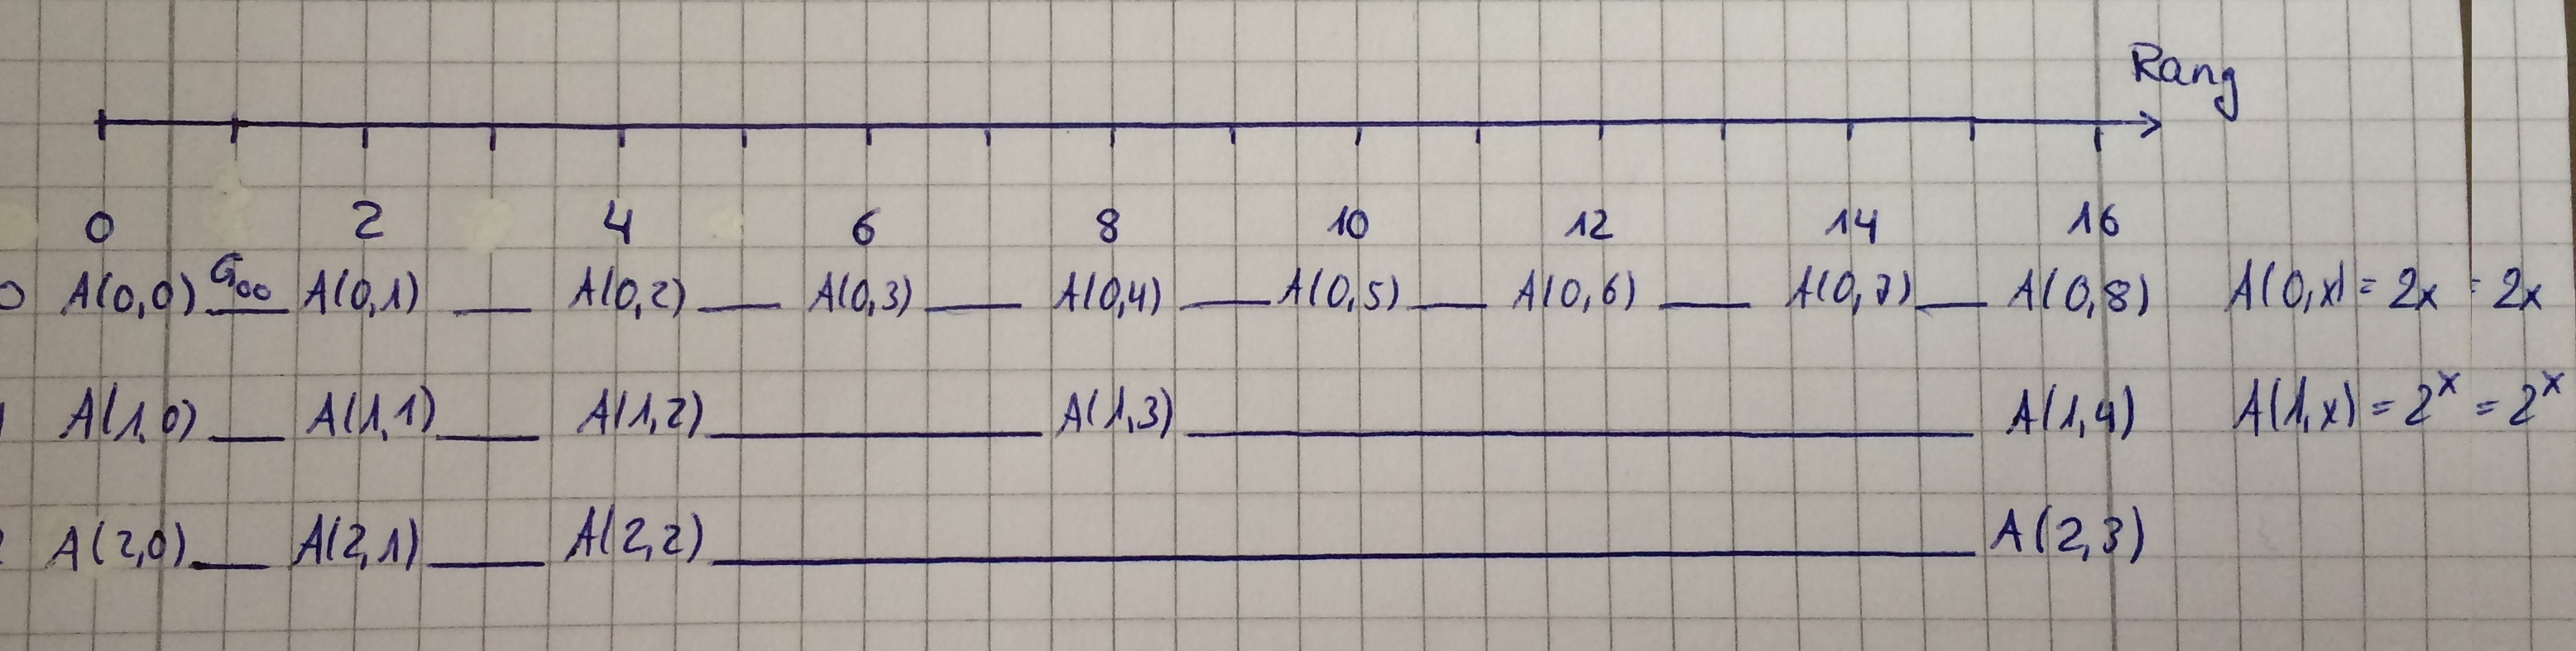
\includegraphics[scale=0.15]{Bild3.png}\\
Beispiel: Rang(x)=7, Rang(y)=13\\
$\Rightarrow$ $x\in G_{0,3},G_{1,2},G_{2,2},...$\\
$\Rightarrow$ $y\in G_{0,6},G_{1,3},G_{2,2},...$\\
Eine Einteilung der Multi-Menge F \\
Für $0\leq k \leq z: N_k=\lbrace (x,y)\in F | k=min\lbrace i\geq 0|\exists j\ mit\ x,y\in G_{i,j}\rbrace\rbrace$\\
und $N_{z+1} := F\setminus\cup_{0\leq i\leq z} N_i$\\
Schließlich definieren wir für $0\leq k\leq z+1: L_k=\lbrace(x,y)\in N_k | (x,y) $ist letzte (oberste) Kante auf PF-Pfad\\
\underline{Lemma:}\\
a) $|L_k| \leq m$ für $0\leq k \leq z+1$\\
b) $|N_0\setminus L_0|\leq n$\\
c) $|N_k\setminus L_k | \leq \frac{5}{8}n$ für $1\leq k \leq z$\\
d) $|N_{z+1}\setminus L_{z+1} | \leq n*a(z,n)$ mit $a(z,n) = min\lbrace i\geq 0 | A(z,i) > log(n)\rbrace$\\
Beweis:\\
a) Für jedes PF gibt es höchstens 1 Kante in $L_k$. Die Behauptung folgt daraus, dass es insgesamt nur m PFs gibt.\\
b) Sei $(x,y)\in N_0\setminus L_0$, dann gilt $\exists j\geq 0$ mit $x,y \in G_{0,j}$, das heißt $A(0,j) \leq Rang(x) < Rang(y) < A(0,j+1)$\\
\hspace*{1cm}$\Rightarrow Rang(x)=2j, Rang(y)=2j+1$\\
\hspace*{1cm}$(x,y) \not\in L_0 \Rightarrow $ nicht die letzte Kante in diesem PF: Betrachte PF von (x,y), dann existiert eine Kante $(s,t)\in L_0$ auf diesem PF-Pfad\\
Situation:\\
$Rang(x)=2j, Rang(y)=2j+1$\\
$Rang(s)\geq Rang(y)$ da letzter Pfad vor dem nicht letzten sein muss\\
$Rang(t) > Rang(s)$ da Pfad von s nach t\\
$\Rightarrow Rang(t) \geq 2j+2$\\
Nach dem PF: x hat neuen Vater (möglicherweise t) u mit $Rang(u)\geq Rang(t)\geq 2k+2$\\
$\Rightarrow$ Rangdifferenz zwischen x und dem neuen Vater u $\geq 2$\\
$\Rightarrow$ Spätere PFs können keine Kante (x,..) mehr zu $N_0$ hinzufügen\\
$\Rightarrow$ Für jeden Knoten wird maximal eine ausgehende Kante (Vaterverweis) in $N_0\setminus L_0$ gezählt werden.\\
$\Rightarrow |N_0\setminus L_0| \leq n$\\
Beweis c), d):\\
Idee: Schätze Beitrag eines Knotens $x\in G_{k,j}$ zu $N_k\setminus L_k$ d.h. alle Kanten, die von x ausgehen und in $N_k\setminus L_k$ gezählt werden.\\
Sei $k\geq 1$ und $x\in G_{k,j}$ beliebig, d.h. $\exists j$ mit $ A(k,j) \leq Rang(x) < A(k,j+1)$\\
und $y_1,...,y_q$ alle Endknoten mit $(x,y_i)\in N_k\setminus L_k$. Ziel: q nach oben abschätzen.\\
$\Rightarrow Rang(y_1)\leq ...\leq Rang(y_q)<A(k,j+1)$\\
Beobachtungen:\\
1) $j\geq 2$ weil sonst k=0 die minimale Zeile definiert, sodass $(x,y_i)$ im selben Intervall ( de ersten 3 Spalten sind immer gleich gefüllt mit 0,2,4). Hier: $k\geq 1$\\
2) $(x,y_i)\not\in L_k$ für $1\leq i\leq q \Rightarrow \exists (s_i,t_i)\in N_k$ auf PF-Pfad von $(x,y_i)$ oberhalb von $(x,y_i)$
Nach der Pfadkopmrimierung ist Vater von $x=y_i+1$. Außerdem ist $y_{i+1}$ Vorfahr von $t_i$ dabei ist $t_i = y_{i+1}$ möglich.\\
%TODO Bild 3: Baum Vorfahren dings
Es gilt stets $Rang(x) < Rang(y_i)\leq Rang(s_i) < Rang(t_i) \leq Rang(y_{i+1}$\\
Definition von $N_k$ k minimal $\Rightarrow (x,y_i),(s_i,t_i)\not\in N_{k-1}$\\
$\Rightarrow \exists j$ mit $Rang(s_i) < A(k-1,j) \leq Rang(t_i)$\\
Daher gilt $Rang(y_i) < A(k-1,j)\leq Rang(y_{i+1})$ für $1\leq i \leq q-1$\\
Anwendung auf di gesamte Folge $y_1,...,y_q$ (d.h. q-1 mal):\\
$Rang(y_1)<A(k-1,j_1)\leq Rang(y_2)<A(k-1,j_2)\leq Rang(y_3)<...\leq Rang(y_{q-1}) < A(k-1,j_{q-1})<Rang(y_q)$\\
Beobachtung: $j_{i+1} \geq j_i \Rightarrow \exists j_1$ mit $Rang(y_1)<A(k-1,j_1)\leq A(k-1,j_1+q-1)\leq Rang(y_q)$\\
$ $\\
\textbf{I.} $\exists j\geq 2: Rang(y_q)\geq A(k-1,j+q-1)$\\
Beweis Teil c:\\
$k\geq 1, x\in G_{k,j},(x,y_i)\in N_k \Rightarrow y_1,...,y_q \in G_{k,j}, j\geq 2$\\
$\Rightarrow A(k,j) \leq Rang(y_1)\leq ...\leq Rang(y_q)<A(k,j+1)$\\
\textbf{II.}$Rang(y_q)<A(k,j+1)$\\
Nach I und II:\\
$\exists j: A(k-1,j+q-1)\leq A(k,j+1) = A(k-1,A(k,j))$\\
$\Rightarrow (Monotonie\ von\ A\ in\ Zeilen) j+q-1 < A(k,j)$\\
$\Rightarrow (j\geq 2) q < A(k,j)$\\
Wir haben gezeigt: Für jeden Knoten $x\in G_{k,j},k\geq 1,j\geq 2$ gibt es höchstens A(k,j) Kanten $(x,y)\in N_k\setminus L_k$\\
$\Rightarrow |N_k\setminus L_k | \leq \sum_{j\geq 2} |G_{k,j} * A(k,j)$ mit $1\leq k \leq z$\\
Behauptung: $|G_{k,j} | \leq \frac{2n}{2^{A(k,j)}}$ extrem fallend, n Knoten im Baum.\\
Daraus folgt: $|N_k\setminus L_k \leq \sum_{j\leq 2} \frac{2n*A(k,j)}{2^{A(k,j)}}$ wobei $A(k,j) \leq 2^j$, da $k\geq 1$ zweite Zeile.\\
$\leq 2n\sum_{j\geq 2} \frac{2^j}{2^{2^j}} = 2n\sum_{j\geq 2} \frac{1}{2^{2^j-j}} = 2n(\frac{1}{4} + \frac{1}{32}+\frac{1}{2^{12}}+...)$ wobei $(\frac{1}{32}+...)$ mit $\frac{1}{16}$ abgeschätzt wird.\\
$\Rightarrow = \frac{5}{8}n$\\
Beweis der Behauptung $|G_{k,j} | \leq \frac{2n}{2^{A(k,j)}}$\\
Sei l beliebig mit $A(k,j) \leq l < A(k,j+1)$\\
Zähle zuerst alle Knoten mit $Rang(x)=l$. Dafür sei $G_{k,j,l} = \lbrace x\in G_{k,j} | Rang(x) = l$\\
Es gilt:\\
1. Jeder Knoten x mit $Rang(x)=l$ hat mindestens $2^l$ Nachkommen (alle Knoten im Unterbaum mit Wurzel x), nach Lemma weighted Union\\
2. Für $x\neq y$ mit $Rang(x)=Rang(y)$ sind die Nachkommensmengen disjunkt.
1+2: $|G_{k,j,l}| \leq \frac{n}{2^l}$ mit n Gesamtanzahl der Knoten\\
$\Rightarrow |G_{kj}| = \sum_{l=A(k,j)}^{A(k,j+1)-1} | G_{k,j,l}|$\\
$\leq \sum_{l=A(k,j)}^{\inf} \frac{n}{2^l} = n\sum_{l=A(k,j)}^{\inf} \frac{1}{2^l}$\\
$= n (1\frac{1}{2^{A(k,j)}} + \frac{1}{2}\frac{1}{{A(k,j)}}+\frac{1}{4}\frac{1}{{A(k,j)}}+...)$\\
$= n*\frac{2}{2^{A(k,j)}}$\\
Beweis Teil d:\\
$k=z+1$, weighted Union $\Rightarrow Rang(y_q) \leq log(n)$\\
Nach I. für $k=z+1$:\\
$A(z,j+q-1) \leq Rang(y_q)\leq log(n)$\\
$\Rightarrow j+q-1 < \alpha (z,n)$, da $\alpha (z,n)$ minimal mit $A(z,\alpha (z,n))>log(n)$\\
$\Rightarrow q < \alpha (z,n)$ mit $j\leq 2$\\
Also gibt es für jeden Knoten x höchstens $\alpha (z,n)$ Kanten $(x,..)\in N_{z+1}\setminus L_{z+1}$ mit n = Anzahl aller Knoten\\
$\Rightarrow |N_{z+1}\setminus L_{z+1} | \leq n*\alpha (z,n)$\\
\underline{Beweis des Satzes (Tarjan):}\\
Jede beliebige Folge von n-1 Unions und $m\geq n$ Finds hat die Gesamtlaufzeit von \oh{m*\alpha (m,n)}\\
Lemma (Kosten aller Finds): Für jedes $z\geq 0$ gilt:\\
 $|F| = \sum_{k=0}^{z+1} |L_k | + \sum_{k=1}^{z+1} |N_k\setminus L_k | = \sum_{k=0}^{z+1} | L_k | + |N_0\setminus L_0 |+\sum_{k=1}^{z} |N_k\setminus L_k | + |N_{z+1}\setminus L_{z+1}|$\\
 $\leq (z+2)*m +n + \frac{5}{8}n*z* + n*\alpha (z,n)$\\
 Betrachte $z=\alpha (m,n),\ n\leq m$ (jedes z liefert eine obere Schranke)\\
 Dann gilt: \\
 $|F|\leq \mathcal{O}(m*\alpha (m,n))+ n+\mathcal{O}(n*\alpha (m,n))+n*\alpha (z,n)$\\
 $|F|\leq \mathcal{O}(m*\alpha(m,n)+n*\alpha(z,n))$\\
 $\Rightarrow \alpha(\alpha(m,n),n) \leq 4\frac{m}{n}$\\
 $\Rightarrow \leq n*\frac{4m}{n} = \mathcal{O}(m)$\\
 Insgesamt: Kosten aller Find-Operationen sind $|F| = \mathcal{O}(m\alpha(m,n)+m)=\mathcal{O}(m\alpha(m,n))$\\
 Kosten aller Unions: \oh{n}=\oh{m}\\
 Bemerkung:\\
 1) In der Praxis sehr gute Laufzeiten (sehr einfache Algorithmen und Datenstrukturen, $\alpha (m,n) < 4 $ für alle in der Praxis vorkommenden Werte von m,n.\\
 2) Die Schranke $m\alpha(m,n)$ ist scharf, d.h. das Union-Find-Problem hat tatsächlich diese Komplexität.Es gibt Beweise für untere Schranke $\Omega(m*\alpha(m,n))$\\
 3) Optimal...yey.\\
 4) Varianten: Split-Find (für Intervalle), \\
 Union-Split-Find: Split(x) markiere x, Union(x) entfernt Markierung, Find(x) nächste Markierung rechts von x\\

\subsection{Wörterbücher}
Wir kennen balancierte Suchbäume.\\
Problem: Teilmenge $S\subseteq U$ mit U Universum, eventuell linear geordnet.\\ 
Speichere S (Schlüssel) in einer Datenstruktur D mit:\\
D.insert(x) $x\in U,\ S\leftarrow S\cup\{ x \}$\\
D.delete(x) $x\in U,\ S\leftarrow S\setminus \{x\}$\\
D.lookup(x) $x\in U$, testet ob $x\in S$\\
Es soll zusätzlich zum Schlüssel Zusatzinformation gespeichert werden.\\
Wir behandeln 2 Datenstrukturen: Randomisierte Suchbäume, Perfektes Hashing\\
\subsubsection{Randomisierter Suchbaum}
Entwickelt von Seidel/Aragon\\
Idee: Verwende einen Zufallsprozess zur Balancierung von binären Suchbäumen.\\
Vorteile: Sehr einfache Implementierung, geringer Aufwand zur Verwaltung der Balance, effiezient\\
\textbf{Definition} RST(Randomized Search Tree):\\
Sei $S=\{x_1,...,x_n\}$ eine Menge von n Schlüsseln aus einem linear geordneten Universum U.\\
Jedem $x_i \in S$ wird zusätzlich eine Zufallszahl $prio(x_i)$, seine Priorität zugeordnet. Diese Zufallszahlen sind gleichverteilte reele Zahlen aus [0,1] oder praktisch ganze Zahlen aus [0,..,$2^{32}-1$].\\
Ein RST für S ist:\\
1) Ein Knotenorientierter binärer Suchbaum für die Paare $(x_i,prio(x_i))$\\
2) Gleichzeitig ein Maximum-Heap bezüglich der Prioritäten $prio(x_i)$\\
\includegraphics[scale=0.07]{6.jpg}\\
Die Prioritäten auf einem Pfad von der Wurzel zu einem Blatt sind monoton fallend. Die maximale Priorität ist in der Wurzel.\\
1) Sie $x_i$ der Schlüssel mit maximaler Priorität, Erzeuge den Wurzelknoten v mit dem Inhalt $(x_i,p_i)$ mit $p_i$ maximal.\\
2) $v.left \leftarrow (\{x_j | x_j < x_i \})$\\
3) $v.right \leftarrow (\{x_k|x_k > x_i\})$\\
Beobachtung: Degenerierter Baum ist unwahrscheinlich, da er nur auftritt, wenn in der Liste der maximale Schlüssel immer die maximale Priorität hat.\\
Erwartete Höhe (Kosten der Operationen) ist \oh{log(n)}.\\
Alternative Konstruktion:\\
Füge alle Schlüssel in absteigender Reihenfolge bzgl. der Priorität in einen normalen Knoten-orientierten Baum ein. Dabei fügt das Insert den entsprechenden Knoten an die richtige Position bzgl. des Schlüssels ein. Der Baum wird durch eine zufällige (weil Prioritäten zufällig) Folge von Inserts aufgebaut.\\
\underline{Operationen auf einem RST:}\\
1) Lookup(x): Normale Suche im binären Suchbaum. Falls $x\in S$ gilt: \oh{Tiefe(x)}, also maximal \oh{Hoehe(T)}\\
2) Insert(x): Bestimme eine zufällige Priorität $prio(x) \in [0,1]$. Füge einen neuen Knoten (Blatt) v mit Inhalt $(x,prio(x))$ gemäß dem Schlüssel x durch ein normales Insert in den RST ein. Im Allgemeinen wird hier die Heapeigenschaft bzgl. der Prioritäten verletzt. Rotiere deswegen v nach oben, bis $prio(vater(v)) \geq prio(v)$ oder bis $v=Wurzel$\\
Beim Rotieren gibt es zwei Fälle:\\
1. v ist rechtes Kind $\rightarrow$ rotate\_left(vater(v))\\
2. v ist linkes Kind $\rightarrow$ rotate\_right(vater(v))\\
Dabei sind es meistens nur wenige auszuführende Rotationen. Der Fall, dass bis zur Wurzel rotiert werden muss (prio(v) ist neues Maximum) ist selten.\\
3) Delete(x): Lookup(x) liefert Knoten v mit Schlüssel x. Rotiere v nach unten, bis er ein Blatt ist. Lösche diesen dann.\\
Runterschieben des zu löschenden Knotens:\\
\begin{lstlisting}
//Sei pl die Prioritaet des linken Kindes, pr die des rechten.
while v ist kein Blatt do
	if pl > pr und v.right == null
		rotate_right(v)
	else
		rotate_left(v)
	fi
od
\end{lstlisting}
4) Split(y) teilt den Unterbaum von y. $s_1 = \{x\in S | x\leq y\}, s_2=\{x\in S|x>y\}$\\
5) Join($T_1,T_2$): Bildet aus den beiden übergebenen RST einen neuen.($T_1,T_1 sind RST von s_1,s_2$)\\
\hspace*{1cm} Bedingung: $max(s_1)<min(s_2)$\\
\hspace*{1cm} Kontruiere RST mit $max(s_1)<x<min(s_2)$ mit x als Wurzelelement mit unendlicher Priorität. Entferne x mit delete(x).\\
\underline{Laufzeitanalyse:}\\
Wir analysieren die erwarteten Kosten einer Delete-Operation in einem RST mit n Knoten. D.h. für Schlüssel $x_1,..,x_n$, die durch Insert eingefügt wurden. Beobachtung: Insert ist das inverse Delete\\
Sei T ein RST für die Menge $S=\{x_1,..,x_n\}$ mit $x_1<..<x_n$ entstanden durch Folge von Inserts.\\
Betrachte Operation Delete($x_k$) mit $1\leq k \leq n$\\
Allgemeine Situation: $P_k$: Suchpfad nach $x_k$, $L_k$: Rechtes Rückgrat vom linken Unterbaum von $x_k$, $R_k$: linkes Rückgrat vom rechten Unterbaum von $x_k$.\\
Kosten: \oh{|P_k|+|L_k| + |R_k|} mit $P_k$ Lookup, $L_k$ und $R_k$ das Rotieren.\\
\underline{Lemma 1:}
Sei $S=\{x_1,...,x_n\}$ mit $x_i<x_{i+1}$ für $i=1,...,n-1$ und $\{prio(x_i) | i=1,...,n\}$ eine Menge von gleichverteilten reelen Zufallszahlen aus [0,1] abgespeichert in einem RST (Betrachte den Knoten v, der einen beliebigen Schlüssel $x_k$ enthält). Dann gilt:\\
a) $E(|P_k|) = H_k + H_{n-k+1}-1$ H: Harmonische Zahl.\\
b) $E(|L_k|) = 1-\frac{1}{k}$\\
c) $E(|R_k|) = a-\frac{1}{n-k+1}$\\
Wobei $H_k = \sum_{i=1}^k \frac{1}{i}$\\
1) $H_k \leq 1+ln(k)$\\
2) $\sum_{i=0}^{k-1} H_i = k*(H_k -1)$\\
\underline{Beweis Lemma 1:}\\
Betrachte eine Permutation $\Pi : \{1,..,n\} \rightarrow \{1,..,n\}$, die S nach Prioritäten absteigend sortiert, d.h. $prio(x_{\Pi(1)})>prio(x_{\Pi(2)})...$. Dann gilt (Beobachtung):\\
1) Jede der Permutationen $\Pi$ ist gleich wahrscheinlich (da Prioritäten gleichverteilt).\\
2) Man erhält den RST (denselben binären Baum) durch normales Einfügen von $x_{\Pi(1)},..,x_{\Pi(n)}$ in einen normalen binären Suchbaum.\\
3) Dann wächst der Baum nur an den Blättern.\\
Duch die zufälligen Prioritäten ist der RST immer ein zufälliger Baum.\\
Teil a): Suchpfad $P_k$\\
Seien $P_k'$ und $P_k''$ eine Zerlegung von $P_k$: $P_k' = \{v\in P_k | key(v)\leq x_k\}$, $P_k'' = \{v\in P_k | key(v) \geq x_k\}$\\
$w\in P_k''$ war zum Zeitpunkt seiner Einfügung der kleinste aller Knoten mit Schlüssel $\geq x_k$, $v\in P_k$ der größte $\leq x_k$\\
Wir zeigen $E(|P_k'|) = H_k$, sowie $E(|P_k''|) = H_{n-k+1}$, daraus folgt a).\\
Zur Abschätzung von $E(|P_k'|)$ definieren wir ein Spiel:\\
Spiel A: Ziehe zufällige Schlüssel aus $\{x_1,...,x_k\}$ und zähle wie oft der Schlüssel maximal ist. Das Spiel endet, sobald $x_k$ gezogen wird.\\
$A^k = $erwartetes Ergebnis von Spiel A für den Schlüssel $x_k = E(|P+k'|)$\\
Induktion: $A^i = H_i$ für $i<k$ (Erwartungswert: $E=\sum_{X}(prob(x)*value(x))$\\
$A^k = \frac{1}{k}*1 + \sum_{i=1}^{k-1}\frac{1}{k}*(1-A^{k-i}) = \frac{1}{k}\sum_{i=1}^k(1+A^{k-i})=\frac{1}{k}(k+\sum_{i=0}^{k-1} H_i)= 1+\frac{1}{k}(k(H_k -1)) = H_k$\\
$\frac{1}{k}*1$: Im ersten Zug $x_k$, $ \sum_{i=1}^{k-1}\frac{1}{k}*(1-A^{k-i})$im 1. Zug nicht $x_k$ sondern $x_i$ aus $\{x_1,...,x_{k-1}\}$\\
Spiel B: Kandidaten $\{x_k,...,x_n\}$. Ziehe zufällige Elemente und zähle wie oft ein neues Minimum gezogen wird.\\
$B^k = $ Erwartungswert dieser Zahl\\
Behauptung: $B^k = H_{n-k+1}$, Beweis symmetrich zu A (Übung)\\
$\Rightarrow$ Teil a) des Lemmas: $E(|P_k|)=H_k+ H_{n-k+1} -1$. -1, weil $x_k$ doppelt gezählt.\\
Wie in Teil a) können wir annehmen, dass der RST ein normaler binärer Baum mit zufälliger Insert-Reihenfolge $x_\Pi(1),...,x_\Pi(n)$ ist.\\
$L_k:$ Ziehe zufällige Elemente sobald $x_k$ gezogen ist (Trigger). Zähle wie oft ein Element $> x_k$ gezogen wird, das maximal ist.\\
$R_k:$ symmetrisch mit Element $<x_k$ minimal.\\
Spiel C: k Kandidaten $\{x_1,...,x_k\}$\\
$C^k := E(|L_k|) = \frac{1}{k} * A^{k-1}+\sum_{i=1}^{k-1}(\frac{1}{k}C^{k-i})$\\
$C^k = \frac{1}{k}(H_{k-1} + \sum_{i=0}^{k-1}C^i$\\
Trick: schätze $\Delta_j := C^{j+1} -C^j$ ab $\Rightarrow \sum_{i=0}^{k-1}C^k = \sum_{i=1}^{k-1}(\Delta_j)$\\
Betrachte: $(j+1)*C^{j+1}-j*C^j = C^j +H_j-H_{j-1}$\\
$\Rightarrow (j+1)*(C^{j+1}-C^j) = H_j - H_{j-1}$\\
$\Rightarrow \frac{1}{j*(j+1)}=C^{j+1}-C^j$\\
$\Rightarrow \Delta_j = \frac{1}{f}-\frac{1}{j+1}$\\
$C^k = \sum_{j=1}^{k-1}\Delta_j = \sum_{j=1}^{k-1}(\frac{1}{j}-\frac{1}{j+1}) = 1-\frac{1}{k}$\\
Spiel D: Kandidaten $\{x_k,...,x_n\}$, zähle wie oft ein Element nach $x_k$ gezogen wird, das minimal ist.\\
$D^k = \frac{1}{n-k+1}B^{k-1} +\sum_{i=k+1}^n(\frac{1}{n-k+1}D^{i-k}$\\
Satz: Sei T ein RST für eine Menge von n Schlüsseln.\\
1. Die erwartete Laufzeit für Insert, Delete und Lookup ist jeweils \oh{log(n)}\\
2. Die erwartete Zahl der Rotationen bei Insert oder Delete ist $< 2$\\
Beweis:\\
1. Kosten für Lookup: $E(|P_k|)$ nach einem $x_k$\\
Lemma Teil a) $E(|P_k|) = H_k + H_{n-k+1} -1$\\
$\Rightarrow \leq 2H_n = $\oh{ln(n)} = \oh{log(n)}\\
Insert, Delete von $x_k$\\
Kosten \oh{|P_k|=|L_k|+|R_k|)} = \oh{H_k + H_{n-k+1} - 1 +1 - \frac{1}{k}+1 - \frac{1}{n-k+1}} = \oh{H_n} = \oh{log(n)}\\
2. Erwartete Anzahl an Rotationen:\\
$E(|L_k|) + E(|R_k|) = 1-\frac{1}{k} + 1 - \frac{1}{n-k+1} < 2$\\
\subsection{Hashing}
Speicherung dünn besetzter Tabellen / sparse tables\\
Spezielle Wörterbücher, da Schlüssel ganze Zahlen. Es werden keine Vergleiche ($\leq$, $\geq$ etc.) auf der Schlüsselmenge durchgeführt. Es gibt keine lineare Ordnung.\\
Genauer: Verwalte Schlüsselmenge $S\subseteq \{0,..,N-1\}$ mit eventuell dazugehörigen Daten (Satellitendaten).\\
Operationen: Lookup(x), Insert(x), Delete(x)\\
Wie immer gilt $n=|S|$, $N=$Anzahl aller Schlüssel.\\
Triviale Lösung: \\
Verwende ein Feld $T[0...N-1]$ (Tafel). Speichere $x\in S$ (mit seinen Daten) an Tafelposition x, d.h. $T[x] \leftarrow x$\\
Für alle $y  \not\in S: T[y] \leftarrow null (-1)$\\
Lookup(x): return T[x]\\
Problem: Speicherplatz \oh{N}, Ziel \oh{n}\\
Ziel Hashing: Laufzeig \oh{1}, Speicher \oh{n}\\
Hashtable: $T[0...m-1]$ mit m Größe der Tafel $m<<N$\\
Hashfunktion: $h: U \rightarrow \{0,...,m-1\}$ mit Universum $U=\{0,...,N-1\}$. Speichert $x\in S$ an Position h(x)\\
Insert: $T[h(x)] \leftarrow x $(Daten)\\
Lookup(x): Teste on $T[h(x)] == x$\\
Die Hashfunktion entscheided, wie die Tabelle kleiner als die Schlüsselmenge werden kann.\\
Häufig verwendete naive Hashfunktion: $h:x\rightarrow x\ mod\ m$\\
Es treten Kollisionen auf, wenn $h(x)=h(y)$ mit $x\neq y$\\
Kollisionsbehandlung:\\
1. Hashing mit Verkettung (Kollisionsmengen werden in Liste gespeichert und mit abgefragtem Wert abgeglichen)\\
Oft $m < n$. Speichere alle Schlüssel $x\in S$ mit $h(x)=i$ in einer Liste $T[i]$. Meißt wird als Funktion der einfache Modulo verwendet.\\
Lookup(x): Durchsuche Liste von $T[h(x)]$ linear. \oh{1+|T[h(x)]}, worstcase \oh{n}\\
\hspace*{1cm} Erwartete Kosten: \oh{1+\frac{n}{m}} (Übung), Belegungsfaktor $\beta = \frac{n}{m}$ (Erwartete Länge einer Liste T[x]\\
Insert(x): Falls Lookup(x)=null füge x an erste Stelle von $T[h(x)]$ ein. \\
Delete(x): Entfernt x aus der Liste $T[h(x)]$\\
Verbesserung: Immer wenn $\beta >4 $ wird, verdopple die Tafelgröße. 1 sehr teures Insert $\rightarrow$, im Schnitt weiter \oh{1}\\
Bei Delete und kleinem $\beta$ kann Tabelle halbiert werden. 1 sehr teures Delete.\\
2. Hashing mit offener Adressierung (Ausprobieren einer Folge von Positionen)\\
Voraussetzung: $n\leq m$ und damit $\beta \leq 1$\\
Idee: Folge von Hashfunktionen $h_0, h_1,...$: $h_i(x) = (f(x) + i * g(x))\ mod\ m$\\
Mit f,g Hashfunktionen $U\rightarrow \{0,..,m-1\}$\\
f(x) gibt die Startposition an, g(x) verschiebt diese.\\
h(x)=1 heißt Linear Probing.\\
Falls belegt probiere $h_1(x), h_2(x),...,$, bis freie Stelle gefunden.\\
Der Status der Positionen kann in einem zweiten Feld status[0..m-1] gespeichert werden (frei, besetzt, gelöscht).\\
Lookup(x): Durchsuche Folge $T[h_0(x)],T[h_1(x)]...$ bis x gefunden, oder freie Position (dann ist x nicht enthalten)\\
Delete(x): Lookup(x) , markiere Position als frei. Problem: Elemente dahinter unerreichbar.\\
\hspace*{1cm}  Lösung: gelöscht flag im Statusarray. Lookup übergeht diesen und hält nicht, Insert erkennt es als freies Feld.\\
3. Perfektes Hashing (keine Kollision durch injektive Funktion) Voraussetzung $n\leq m$\\
$S\subseteq \{0,...,N-1\} n=|S|$ verwende Tafel der Größe $m\geq n$ und m=\oh{n}\\
Statisch: S ist fest, nur 2 Operationen. Init(S) Konstruktor, Lookup(x)\\
Ziel: Tafelgröße s=\oh{n}, Hashfunktion injektiv auf S\\
Gegeben $S\subseteq \{0,..,N-1\}$ und Tafel $T[-,...,s-1]$\\
Injektive Funktion $h:\{0,...,N-1\} \rightarrow \{0,...,s-1\}$ injektiv auf S\\
Idee: Verwende ein randomisiertes Verfahren, d.h. wähle eine zufällige Funktion aus den Kandidaten.\\
Originalarbeit: Storing a Sparse Table with \oh{1} worst-case Access Time\\
Verwende zweistufiges Hashing Schema (injektiv), Auswahl der Funktion durch Randomisierung\\
1. Schritt: Funktion (muss noch nicht injektiv sein) bildet auf eine Liste von Buckets ($W_0,...,W_{s-1}$) $W_i=\{x\in S | h(x)=i\}$ ab, mit s der Größe der ersten Stufe.\\
2. Schritt: Für jedes $W_i$ gibt es eine eigene Hashfunktion $h_i$, die jeweils auf eine weitere Tafel der Größe s abbilden. $h_i$ ist injektiv auf $W_i$. Für jedes $W_i$ gibt es eine eigene 2. Tafel $\{m_0,...,m_{s-1}\}$. Dadurch gibt es auf der zweiten Stufe quadratische Tafelgröße.\\
Man findet "leicht" eine Funktion h der ersten Stufe mit $\sum_{i=0}^{s-1} |W_i|^2 = $\oh{n}\\
Für Tafeln quadratischer Größe findet man relativ leicht injektive Hashfunktion.
Sei p eine Primzahl mit $p>N$. $U=\{0,...,N-1\}, S\subseteq U,n=|S|$, $s\in\mathbb{N}$ Tafelgröße\\
Betrachte folgende Hashfunktionen $h_1,...,h_{p-1}$\\
$h_k:\{0,...,N-1\} \rightarrow \{0,...,s-1\}$\\
$h_k(x) = (k*x\ mod\ p)\ mod\ s$\\
Jede Funktion $h_k, 1\leq k\leq p-1$ veteilt die Menge S auf s Buckets:\\
$W_0^k,...,W_{s-1}^k$, d.h. genauer: $W_i^k = \{x\in S|h_k(x)=i\}$\\
Lemma1: Für jede Menge $S\subseteq \{0,...,N-1\}$ mit $|S|=n$ gilt:\\
$\exists k, 1\leq kleq p-1$ mit $\sum_{i=0}^{s-1}({|W_i^k| \choose 2})<\frac{n^2}{s}$\\
$({n \choose k}) = \frac{n!}{k!(n-k)!}$: Anzahl der k-elementigen Teilmengen einer Menge der Größe n\\
$({n \choose 2}) = \frac{n*n-1}{2}$\\
hier: $({|W_i^k| \choose 2})$: Anzahl aller $\{x,y\} x\neq y, x,z\in S$, die im selben Bucket $W_i^k$ landen. (\#Kollisionen)
Beweis:\\
Behauptung: $\sum_{k-1}^{p-1}\sum_{i=0}^{s-1}({|W_i^k| \choose 2}) < (p-1)\frac{n^2}{s}$ (Beweis später)\\
Daraus folgt Lemma1. Indirekt gilt Lemma 1 nicht $\Rightarrow \forall 1\leq k\leq p-1: \sum_{i=0}^{s-1}({|W_i^k| \choose 2}) \geq \frac{n^2}{s}\Rightarrow \sum_{i=1}^{p-1}\sum_{i=0}^{s-1}({|W_i^k| \choose 2}) \geq (p-1)\frac{n^2}{s} $Widerspruch zu Behauptung\\
Folgerung 1: Für $s=n$ (d.h. Tafelgröße n) folgt aus Lemma1: $\exists k, 1\leq k\leq p-1: \sum_{i=0}^{n-1}(|W_i^k|^2)<3n$\\
Beweis: Betrachte Lemma1 für s=n\\
$\exists 1\leq k\leq p-1 :\sum_{i=0}^{n-1}({|W_i^k| \choose 2}) < n$\\
$\sum_{i=0}^{n-1}\frac{|W_i^k|*(|W_i^k|p1)}{2} < n$\\
$\sum_{i=0}^{n-1}|W_i^k|(|W_i^k|-1) <2n$\\
$\sum_{i=0}^{n-1}(|W_i^k|^2-|W_i^k|) <2n$\\
$\sum_{i=0}^{n-1}|W_i^k|^2 < 2n+\sum_{i=0}^{n-1} |W_i^k|$ wobei $\sum_{i=0}^{n-1} |W_i^k| = n$ also $|S|$\\
Folgerung 2: Für $s=n^2$ foglt aus Lemma 1: $\exists 1\leq k' \leq p-1$ sodass die Hashfunktion $h_{k'}:x\rightarrow (k'*x\ mod\ p)\ mod\ n^2$ die injektiv auf S ist, d.h. $|W_i^{k'}|\leq 1$ für $i=0,...,n^2-1$\\
Für quadratische Tafelgrößen existiert eine perfekte Hashfunktion $h_{k'}$\\
Beweis: Betrachte Lemma 1 für $s=n^2$\\
$\exists 1\leq k'\leq p-1$ mit $\sum_{i=0}^{n-1}({|W_i^{k'}| \choose 2}) < \frac{n^2}{2}=1\Rightarrow \sum_{i=0}^{n^2-1}({|W_i^{k'}| \choose 2}) = 0 \Rightarrow \forall 0\leq i \leq n^2-1: |W_i^{k'}|\leq 1 \Rightarrow \#Kollisionen=0$\\
Vermeidung des quadratischen Speicherplatzes durch ein 2-Stufiges hashing-Schema.\\
1. Stufe: Verwende Tafelgröße s=n und wähle ein k gemäß der Folgerung d.h. $\sum_{i=0}^{n-1}|W_i^k|^2<3n$\\
Die Hashfunktion $h_k(x):x\rightarrow (kx\ mod\ p)\ mod\ n$ verteilt s auf eine Tafel der Größe n, sodass die Summe der Quadrate der Bucketgrößen kleiner ist als 3n.\\
2. Stufe: Für jedes nicht-leere Bucket $W_i^k$ der 1. Stufe verwende eine Tafel der Größe $s_i=|W_i^k|^2$ und wähle $k_i$ gemäß Folgerung 2. Genauer: Für i=0,...,n-1 wähle ein $k_i$ sodass $h_{k_i}(x): x\rightarrow (k_ix\ mod\ p)\ mod\ s_i$ injektiv auf $W_i^k$ ist.\\
Gesamtbedarf: 1. Stufe: Platz n, 2. Stufe: $\sum_{i=0}^{n-1}|W_i^k|^2 < 3n$ ungefähr $4n$, genauer später.\\
Problem: Wie findet man diese injektiven Funktionen, d.h. wie wählt man k und $k'$\\
Idee: Erhöhe die Tafelgrößen auf Stufe 1 und Stufe 2 um einen konstanten Faktor. Dann erfüllen mindestens 50\% aller k die Bedingungen von Folge 1\&2\\
Beweis der Behauptung:\\
(*)$\sum_{k=1}^{p-1}\sum_{i=0}^{s-1} {|W_i^k| \choose 2})<(p-1)\frac{n^2}{s}\Rightarrow \exists k:\sum_{i=0}^{s-1}({|W_i^k| \choose 2})<\frac{n^2}{s}$\\
Mit p Primzahl $p\geq N$
Die Summe ist: Anzahl aller Paare $(l,\{x,y\})$ mit $1\leq k \leq p-1,\ x,y\in S,\ x\neq y$ und $h_k(x) = h_k(y)$ (Kollision).\\
Beitrag eines festen Paares $x\neq y$ zu der Summe = Anzahl aller k mit $h_k(x)=h_k(y)$\\
$(kx\ mod\ p-ky\ mod\ p)\ mod\ s = 0$\\
$kx\ mod\ p-ky\ mod\ p = i*s\ i\in \mathbb{Z}$\\
$k*(x-y)\ mod\ p\in \{-(p-1),...,p-1\}$ Vielfaches von s aus der Menge $\Rightarrow \frac{2*(p-1)}{s}$ verschiedene Gleichungen\\
Lösen der Gleichung nach k $k=\frac{i*s}{x-y}\ mod\ p)$ Da p eine Primzahl ($\mathbb{Z_p}$ ein Körper) existiert eine wohl-definierte Division (inverse zur Multiplikation) und daher besitzt jede Gleichung höchstens eine Lösung für k.\\
$\Rightarrow$ Der Beitrag von \{x,y\} $x\neq y$ zur Summe $\leq \frac{2(p-1)}{s}$\\
Wir summieren über  alle 2-elementigen Teilmengen $\{x,y\}, x\neq y, x,y\in S$:\\
Anzahl der Teilmengen (*) $\leq ({n \choose 2}) * \frac{2(p-1)}{s}=\frac{n(n-1)}{2}*\frac{2(p-1)}{s}\leq n^2\frac{p-1}{s}$\\
Implementierung Beispiel:\\
3 Felder (1. Stufe) $W[0...n-1]$ mit $W[i]$ Pointer auf Bucket 2. Stufe.\\
\hspace*{1cm}size]-...n-1] Anzahl aller Elemente in $W_i^k$\\
\hspace*{1cm} $K[0...n-1]$ mit $K[i]=k_i$ k-Werte der 2. Stufe.\\
\hspace*{1cm} Variable $k_0 = $k der ersten Stufe\\
Für 2. Stufe: n Tafeln $B_i$ mit $i=0...n-1$ und $B_i[0...size[i]^2-1]$\\
Platzbedarf: $size+K+W+k_0+B_i = 3n+1\ +\ \sum_{i=0}^{n-1} size[i]^2 \leq 6n+1 =$\oh{n}\\
Speichere $x\in S$ wie folgt: $i\leftarrow h_{k_0}(x),\ j\leftarrow h_{K[i]}(x),\ W[i][j] \leftarrow x$\\
Mit $h_{k_0} = ((k_0*x\ mod\ p)\ mod\ n$ und $h_{K[i]}(x) = ((K[i] * x)\ mod\ p)\ mod\ size[i]^2$\\
Lookup: Teste ob W[i][j]==x\\
Bemerkung: Für size[i]=0 kein $B_i$ auf 2. Stufe, W[i]=null; Für size[i]=1 keine neue Hashfunktion K[i], speichere direkt.\\
\hspace*{1cm} Für kleine size[i] konstant kann man Verkettung anstelle von Hashfunktion+Tabelle nehmen.
Aufbauzeit: \oh{n*N} für Garantie eines k (alle k ausprobieren)\\
Randomisierung: Wir brauchen viele geeignete k's, dann ist mit hoher Wahrscheinlichkeit ein zufällig gewähltes gut.\\
Folgerung 3: Für $s=n$ in Lemma 1 gilt für mindesetens die Hälfte aller k $1\leq k\leq p-1$ $\sum_{i=0}^n |W_i^k|^2 < 5n$\\
Beweis: $\sum_{k=1}^{p-1}\sum_{i=0}^{s-1}({|W_i^k| \choose 2}) < (p-1)\frac{n^2}{s}$\\
$\sum_{k=1}^{p-1}\sum_{i=0}^{n-1}({|W_i^k| \choose 2}) <(p-1)n$\\
Anhand der Behauptung hälfte aller ks: $\sum_{i=0}^{n-1}({|W_i^k|\choose 2}) < 2n$ denn sonst ist für mehr als die hälfte der Wert $\geq 2$\\
(2n ist ungefähr der Mittelwert der $W_i^k$'s.\\
$\Rightarrow \sum_{i=0}^{n-1} \frac{|W_i^k|(|W_i^k|-1)}{2}<2n$\\
\hspace*{1cm}$\sum_{i=0}^{n-1} |W_i^k|^2 - \sum_{i=0}^{n-1} |W_i^k| < 4n$
Da $\sum_{i=0}^{n-1} |W_i^k| = n$: $\sum_{i=0}^{n-1} |W_i^k|^2<5n$\\
Folgerung 4: Für $s=2n^2$(Lemma 1) gilt für mindestens die Hälfte aller k' $1\leq k'\leq p-1$: $h_{k'}(x)\rightarrow (k'x\ mod\ p)\ mod\ 2n^2$ ist injektiv auf S.\\
Beweis: $s=2n^2$: $\sum_{k=0}^{p-1}\sum_{i=0}^{2n^2-1} ({|W_i^k| \choose 2}) < (p-1) \frac{n^2}{2n^2} \Rightarrow <\frac{1}{2}(p-1)$\\
Daraus folgt, dass für mindestens die Hälfte aller k $1\leq k\leq p-1$ gilt: $\sum_{i=0}^{2n^2-1}({ |W_i^k| \choose 2}) = 0$ (das entsprechende $h_k$ ist injektiv.\\
Platzbedarf: 1. Stufe:$3n+1$, 2. Stufe: $\sum_{i=0}^{n-1}2|W_i^k|^2 = 2\sum_{i=0}^{n-1}|W_i^k|^2 < 10n$. Insgesamt 13n+1=\oh{n}\\
Randomisierte Berechnung der k-Werte. Mindestens die Hälfte sind geeignet. Dann ist zufälliges k mit Wahrscheinlichkeit $\frac{1}{2}$ ok. $\Rightarrow$ Erwartete Anzahl von zufälligen Ziehungen bis ein k gefunden ist ist 2. Erwaretete Aufbauzeit \oh{n}\\
Zusammenfassung (Perfect Hashing): Jede Menge $S\subseteq \{0,...,N-1\}$ mit $|S|=n$ kann so abgespeichert werden, dass gilt:\\
\hspace*{1cm}1: Platzbedarf ist \oh{n} (13n)\\
\hspace*{1cm}2: Erwartete Aufbauzeit ist \oh{n}\\
\hspace*{1cm}3: Zugriff (Lookup) in Ziet \oh{1} im worst-case\\
Dynamisierung (Insert/Delete) ist möglich (Dynamic perfect hashing)\\
Bei Kollisionen (unwahrscheinlich) muss Tafels 2. Stufe neu gebaut werden (Rehashing)\\
\subsection{Priority Queues}
Definition des Datentyps: Priority Queue PQ speichert Paare (p,i) von Prioritäten und Informationen $p\in P, i\in I$\\
z.B. P ganze Zahlen, I Knoten eines Graphen\\
Operationen: PQ.insert(p,i) fügt das Paar (p,i) ein. PQ.findmin() liefert ein Paar mit minimaler Priorität. PQ.delmin() entfernt das Paar PQ.findmin(). PQ.decrease\_p(x,q) vermindert die Priorität des Paares x=(p,i) auf q d.h. (q,i) mit $q<p$\\
\subsubsection{Mögliche Implementierung}
1. Unsortierte Liste: Liste speichert Wert und Priorität, Insert/Decrease=O(1), Find=O(n)\\
2. Sortierte Liste (Suchbaun)\\
3. Fibonacci Heap\\
\subsubsection{Amortisierte Analyse Fibonacci Heap}
Abschätzung einer beliebigen Folge von Operationen auf einer Datenstruktur D: $D_0\rightarrow^{op_0}D_1\rightarrow^{op_1}D_2...$\\
Die amortisierten Kosten sind die durchschnittlichen Kosten einer beliebigen Operation. (Hier Gesamtkosten / n)\\
Beispiel: Binärzähler mit den Operationen Init (Setze auf 0) und Increase (erhöhe um 1)\\
Datenstruktur: Bitstring $...a_3a_2a_1a_0$ mit $ a_i\in \{0,1\}$\\
Zählerwert = $\sum_{i\geq 0}a_i2^i$\\
Operationen: Init: Erzeuge Liste der Länge 1 mit $a_0=0$. Kosten \oh{1}\\
Increment:\\
$a_0\leftarrow a_0+1$\\
$i=0$\\
while $a_i=2$ do\\
$a_i=0;a_{i+1}\leftarrow a_{i+1}+1;i\leftarrow i+1;$\\
done\\
Increment Laufzeit: \oh{1+\text{Anzahl Überträge}}
Laufzeit einer Folge Init und n Increment: \oh{n*log(n)} (worst case), da die Zahl log(n) Bits hat.\\
Da so hohe Überträge sehr selten sind eher \oh{n}
\subsubsection{Amortisierte Analyse: Potentialmethode}
Allgemein: Datenstruktur D, Potential (Funktion $pot:D\rightarrow R_0^+$\\
Operation: $op: D'\rightarrow^{op}D''$\\
Definition: $T_{\text{Tats}}(op): $ Ausführungszeit einer Operation (Tatsächliche Kosten)\\
\hspace*{1cm} $T_{\text{Amort}}(op) = T_{\text{Tats}}(op)+pot(D'')-pot(D')$\\
\hspace*{1cm} D.h.:$T_{\text{Amort}}(op) = T_{\text{Tats}}(op)+\Delta pot$\\
Betrachte nun eine Folge von n Operationen: $D_0\rightarrow^{op_0}D_1\rightarrow^{op_1}D_2\rightarrow^{op_n}D_n$\\
Dann gilt: $\sum_{i=1}^n T_{\text{Tats}}(op_i) = \sum_{i=1}^n T_{\text{Amort}}(op_i) + pot(D_0) - pot(D_n)$\\
Spezialfall: $pot(D_0) = 0; pot(D_i)\geq 0 \Rightarrow \sum_{i=1}^n T_{\text{Tats}}(op_i) \leq \sum_{i=1}^n T_{\text{Amort}}(op_i)$
Anwendung auf Zähler (INIT$\rightarrow D_0 \rightarrow^{increment} D_1...$):\\
Problem: Wähle gut Potentialfunktion, die eine gute Schranke liefert.\\
Hier: pot = Anzahl aller 1 im Bitstring. Bedingung des Spezialfalls erfüllt.\\
Betrachte nun $T_{\text{Tats}}$ und $T_{\text{Amort}}$\\
Wenn der Zähler nun folgende Form hat: $xxx0111$ mit der ersten Null von rechts aus gesehen und k Einsen davor, dann ist:\\
1. $T_{\text{Tats}}(incr)=$\oh{1+k}\\
2. $\Delta pot=1-k$\\
Also: $T_{\text{Tats}}(incr)=1+k + (1-k )= 2 =$\oh{1}\\
$\Rightarrow$ Potentialmethode Gesamtkosten 2n = \oh{n}
\subsubsection{Fibonacci Heaps}
Warteschlangen werden realisiert durch eine Menge sogenannter "Heap ordered Trees".\\
Ein Baum T heißt "Heap ordered", wenn seine Knoten mit Prioritäten beschriftet sind, sodass  für alle Knoten $v\neq $Wurzel gilt: prio(v)$\geq$ prio(vater(v)).\\
Wir benötigen einige Pointer in den Knoten: Vater, Verweise auf 1. Kind, alle Kinder eines Knoten in zyklischer doppeltverketteten Liste (2 Verweise im Knoten), und Daten\\
Mögliche Klasse:\\
\begin{lstlisting}
class node{
	P prio;
	I indo;
	node parent,left_sib,right_sib;
	bool mark;
	int rank
}
\end{lstlisting}
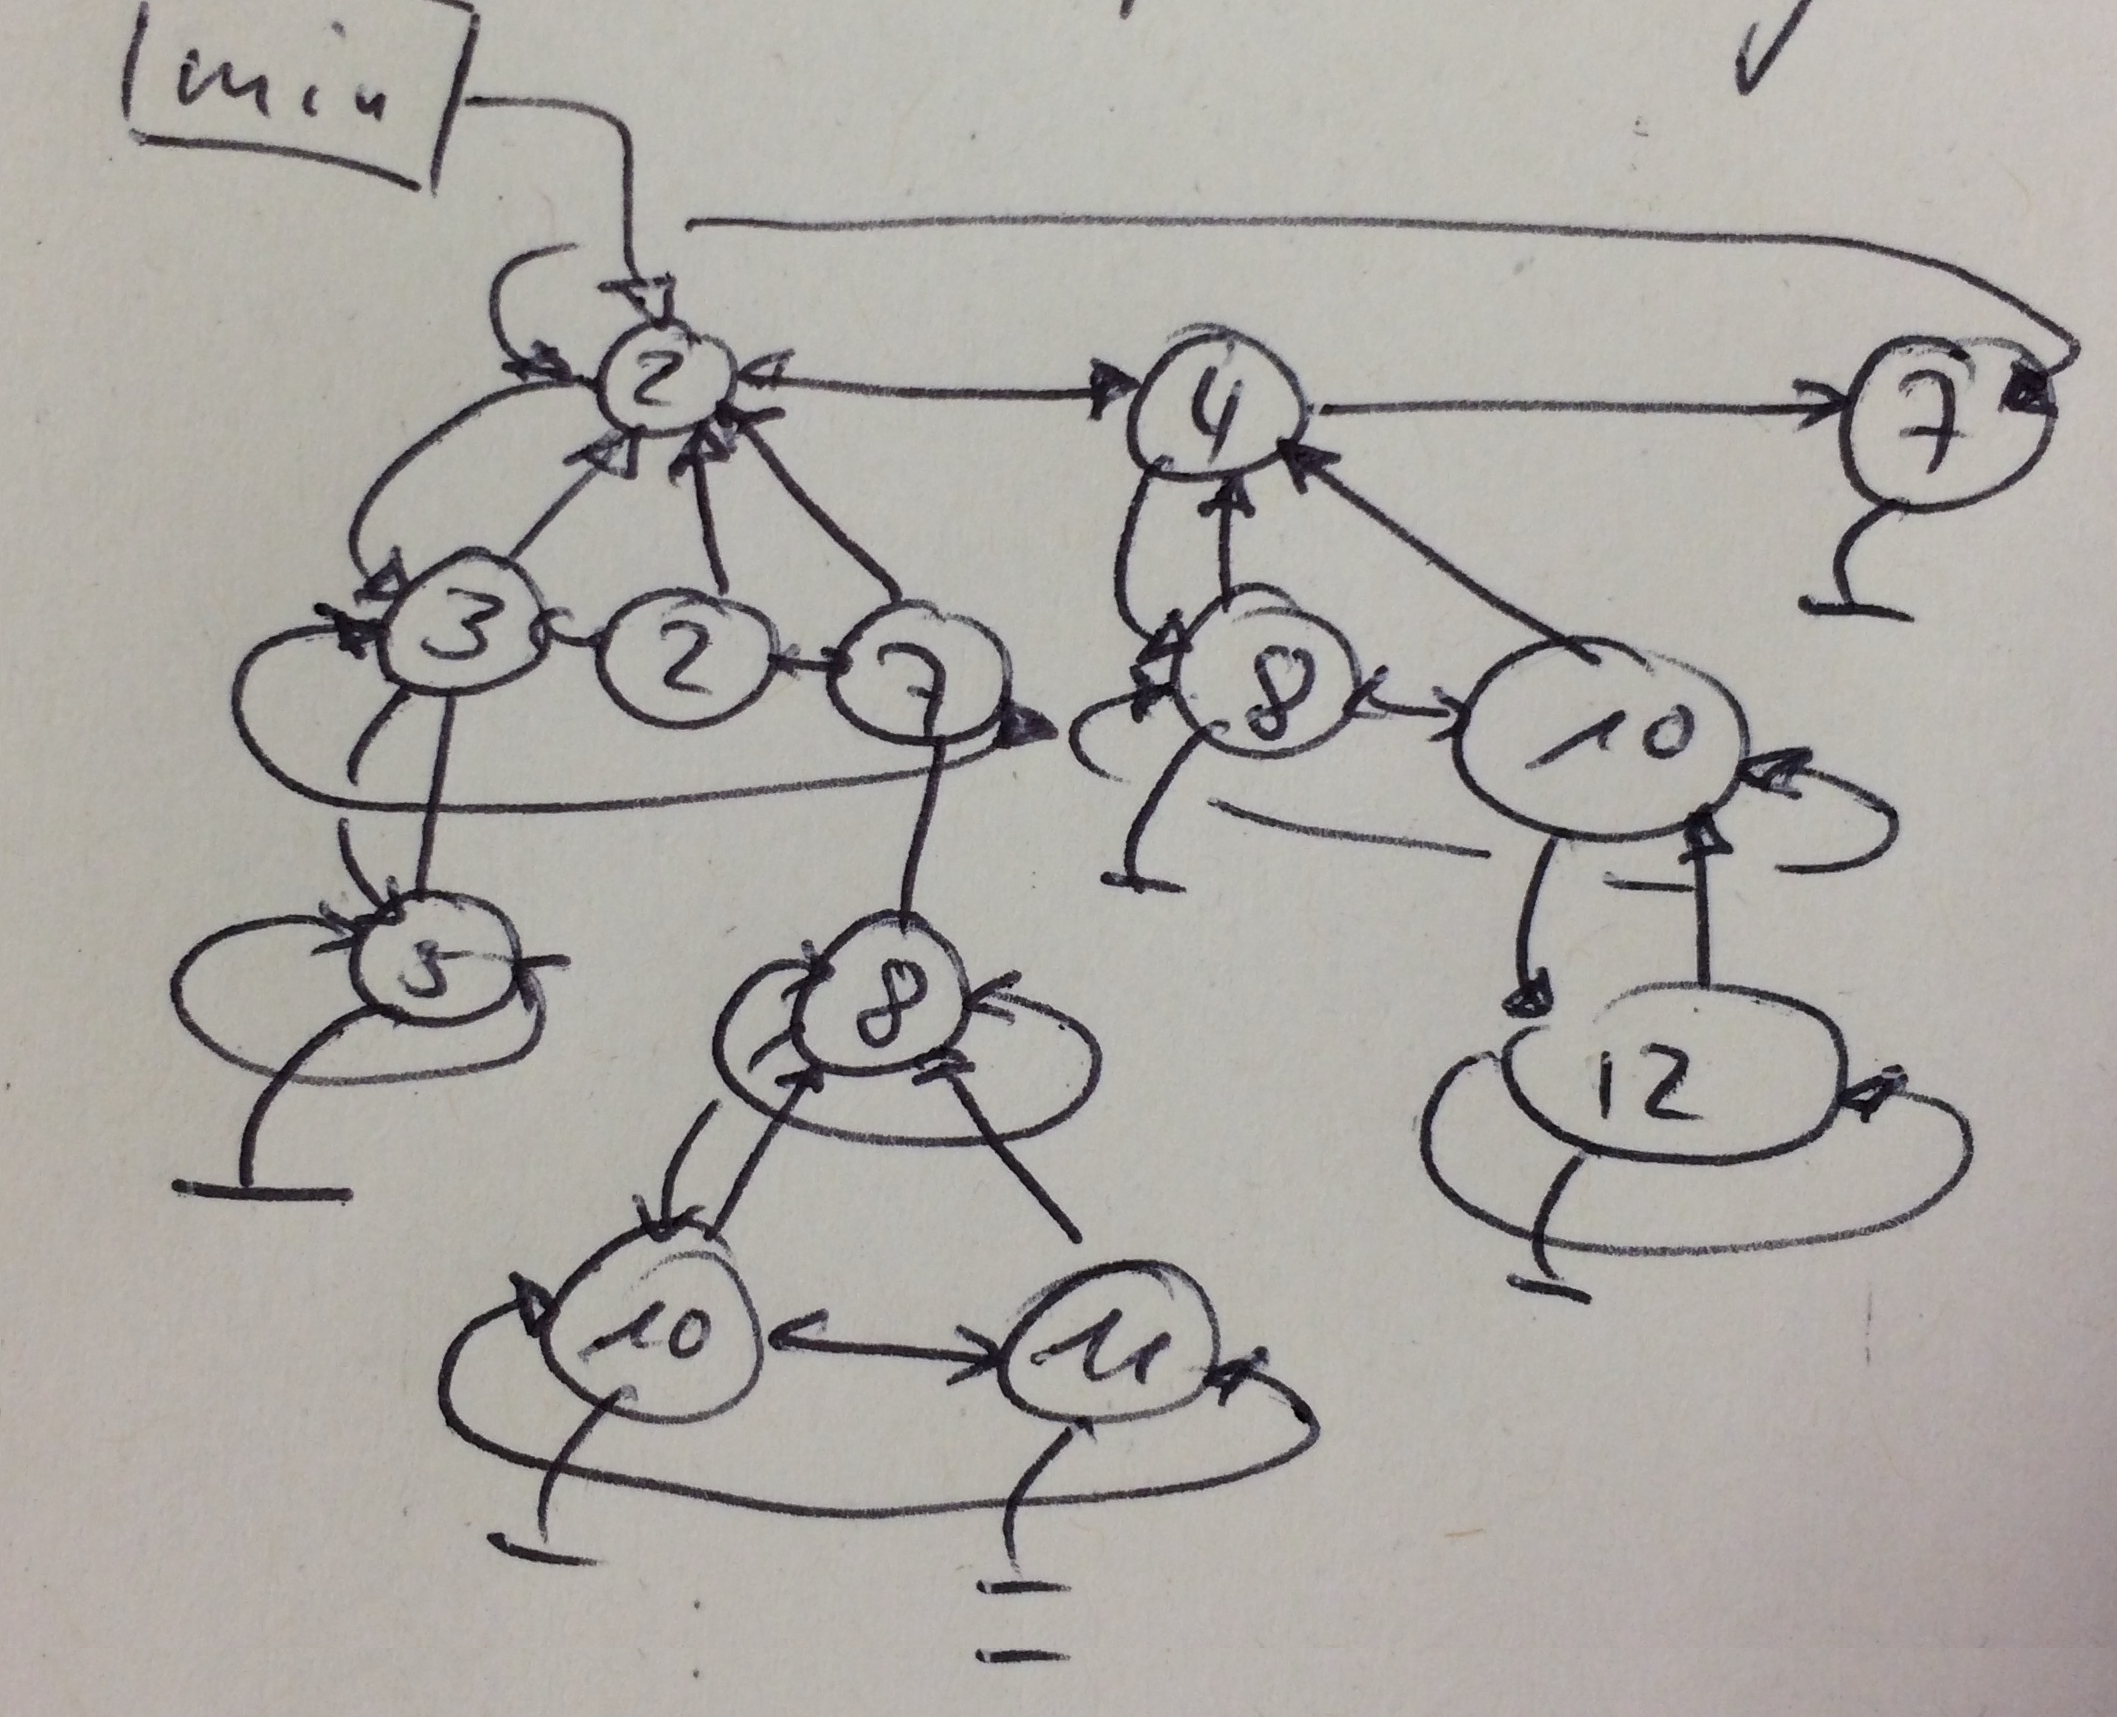
\includegraphics[scale=0.1]{7.png}\\
Auch Wurzel ist in einer zyklischen Liste (Wurzelliste).\\
Realisierung der Operationen:\\
Konstruktor(Init)\oh{1}: min=0\\
PQ.findmin()\oh{1}: Zugriff über min\_pointer\\
PQ.insert(p,i)\oh{1}:  Erzeuge neuen Baum, der nur aus 1 Knoten besteht. Füge v in die Wurzelliste dieses Baums ein, v.prio = p, v.info = i. Falls $p<minprio$ dann min=v\\
PQ.delmin(): Bringt Fib.-Heap in eine besondere Form: 
Alle Wurzeln sollen paarweise unterschiedliche Rängehaben (\# Kinder).\\
delmin im Detail:\begin{enumerate}
\item[1.] $v\leftarrow min$
\item[2.] Lösche v aus der Wurzelliste (doppelt verkettet) und füge alle Kinder v in die Wurzelliste ein. (Hier entstehen gleiche Ränge. \oh{rang(v)}
\item[3.] Eliminiere Mehrfach-Vorkommen des gleichen Rangs:\\
while $\exists$ 2 Wurzeln $v_1,v_2$ gibt, sodass $v_1\neq v_2$ und rang($v_1$)=rang($v_2$)\\
do: If $v_1.prio\leq v_2.prio$, sonst vertausche ; Verschmelze($v_1,v_2$) (Mache $v_2$ zum Kind von $v_1$)\\
(Hänge Baum größerer Priorität an den der kleineren Priorität)\\
Daraus folgt: Alle Wurzeln haben verschiedenen Rang $\Rightarrow$ \# Wurzeln $\leq$ max Rang.\\
Kosten: \oh{maxRang}\\
\item[4.]Lineare Suche nach Minimum
\end{enumerate}
Lemma: Schritt 3 hat Laufzeit $T_{\text{Tats}}$ \oh{maxRang + \# Verschmelzungen}\\
Beweis: durch Algorithmus\\
Idee: Verwende Feld (Tafel) Rank[0,...,maxRang]. Speichere in Rank[i] die Wurzel mit Rang=i (unter allen bereits bearbeiteten Wurzeln)
\begin{lstlisting}
for i=0 to maxRang do Rank[i] = null od
forall wurzel v in Wurzelliste do
	while Rank[rang(v)] != null do
		vtmp = Rank[rang(v)]
		Rank[rang(v)] = null
		v = Verschmelze (v,vtmp)
	done
	Rank[rang(v)]=v
done
\end{lstlisting}
Laufzeit: Sei \# $W_0$ = \# Wurzeln vor z.2; \# $W_1$ = \# Wurzeln nach z.2; \# V=\# Verschmelzungen \\
Dann gilt: \\
1. Laufzeit von z.2 \oh{maxRang + \# W_0 + \# V}\\
2. \# $W_0$ = $\# W_1 + \# V$ Weil jede Verschmelzung eine Wurzel eliminiert\\
3. Am Ende ist \# $W_1\leq maxRang$ da alle Ränge verschieden)\\
$\Rightarrow$ \oh{maxRang +\# W_0 + \# W_1} = \oh{maxRang + \# W_1 + \# V + \# W_1} = \oh{maxRang + \# W_1 + \# V} = \oh{maxRang+\# V}\\
Da $\# W_1 \leq maxRang$. Es bleibt abzuschätzen was maxRang und \# V ist.\\
Wir schätzen den maximalen Rang ab. Beobachtung Insert,Delmin erzeugen spezielle Bäume (binomische Bäume).\\
Folge von Bäumen: $T_0,...,T_i$ mit $T_0$ ein Knoten, $T_{i+1}$ ist $T_i$ mit einem weiteren $T_i$ als zusätzliches Kind.\\
Der Maximale Rang ist an der Wurzel. Anzahl der Knoten verdoppelt sich mit steigendem i, Rang erhöht sich um 1.\\
Lemma: maxRang = log(n) in binomischen Bäumen, wobei n die Anzahl der Knoten ist.\\
Beweis: 1. Die Wurzel von $T_i$ hat Rang i, $T_i$ hat $2^i$ Knoten (verdoppelt sich in jedem Schritt $i\rightarrow i+1$\\
\hspace*{0.5cm}$\Rightarrow$ Wurzel hat Rang log(n).\\
\hspace*{0.5cm}2. Wurzel hat maximalen Rang in $T_i$, da alle Nachkommen Wurzen von $T_j$ sind, mit $j<i$. 2. Folgt aus 1.\\
Fibonacci-Heap ist eine Menge von binomischen Bäumen. Nach Lemma gilt maxRang$\leq log(n)$ wobei n Anzahl der Knoten ist.\\
Amortisierte Analyse:\\
\hspace*{0.5cm} Potential = Anzahl der Wurzeln.\\
$T_{\text{amort}}(op)=T_{\text{tats}}(op) + \Delta pot$\\
Betrachte beliebige Folge von Operationen. Dann sind:\\
create=\oh{1}, finMin=\oh{1}, da $T_{\text{tats}}=$\oh{1} und $\Delta pot=0$.\\
insert: $T_{\text{tats}}=$\oh{1} und $\Delta pot=1 \Rightarrow T_{\text{amort}}=$\oh{1}\\
delmin: $T_{\text{tats}}=$\oh{maxRang+\#V}. $\Delta pot \leq $maxRang $-\#V$, wobei die Kinder von v zu Wurzeln werden und jede Verschmelzung eine Wurzel entfernt\\
\hspace*{0.5cm} $T_{\text{amort}} = T_{\text{tats}}+\Delta pot \leq maxRang +\#V + maxRang -\#V=2maxRang = $\oh{log(n)}\\
Bemerkung: Amortisierte Analyse kann auch modelliert werden durch sogenannte "coin operated machines". Das Potential wird dabei als eine Art Konto angesehen. \\
Eine beliebige Folge von $n_1$ Inserts, $n_2$ FindMins, $n_3$ DelMins und 1 Create hat Gesamtkosten \oh{n_1+n_2+n_3*log(n)}\\
Worstcase Kosten von delMin sind \oh{n}\\
Wir behandeln nun PQ.decrease(v,q): v Knoten, q neue kleinere Priorität.\\
Schritte:\begin{enumerate}
\item[1] v.prio = q (verminderung), verletzt u.U. die Heap-Eigenschaft \oh{1}
\item[cut] Lösche den Pointer zum Vaterknoten und füge v in die Wurzelliste ein (und aus Geschwisterliste löschen), Kinderknoten hängen weiterhin an v, setze v.mark=false \oh{1}
\item[3] Update des min-Pointers für minimale Wurzel \oh{1}

\end{enumerate}
Achtung: Baum ist nicht mehr binomisch $\rightarrow$ log(n) Schranke für maxRang ist nicht mehr gültig\\
Wie kann man den Rang dennoch auf log(n) beschränken:\\
Idee: Setze das Löschen von Vaterverweisen in Richtung Wurzel fort, sobald ein zweites Kind entfernt wird:
\begin{enumerate}
\item[4] Falls v keine Wurzel, Markiere(Vater(v))
\end{enumerate}
\begin{lstlisting}
Markiere(v):
while w.parent!=null UND w.mark=true do
	u=w.parent
	Fuege w in Wurzelliste ein
	w.mark = false
	w=u
done
if w.parent!=null then
	w.mark=true
fi
\end{lstlisting}
Wurzeln sind stets unmarkiert.\\
Beobachtung: Eine decrease-Operation kann sehr viele cut-Operationen zur Folge haben.\\
Wie zeigen, dass durch diese Markierungsstrategie den maximale Rang durch \oh{log(n)} beschränkt.\\
Lemma: MaxRang $\leq 1,4404* log(n)$\\
Beweis: Idee: Zeige, dass \# Knoten expotentiell mit maxRang wächst (untere Schranke) $\Rightarrow $maxRang=\oh{log(n)}\\
Sei v beliebiger Knoten mit Rang i. Ordne die Kinder von v nach der Zeit, zu der sie am Knoten v angehängt wurden (Verschmelzung)\\
Sei $w_j$ das j. Kind.\\
Behauptung: $Rang(w_j)\geq j-2$\\
Beweis: Als $w_j$ Kind von v wurde galt: $Rang(w_j)=j-1$. $w_j$ hat seitdem höchstens 1 Kind verloren (da er nicht Wurzel ist, Markierungsstrategie) $\Rightarrow Rang(w_j)\leq j-2$\\
Sein nun v ein Knoten mit Rang i und $s_i := $minimale Zahl von Knoten um Unterbaum mit Wurzel vom Rang i.\\
$s_0=1; s_1=2$ trivial. Für $i>2: s_i=2+s_0+...+s_{i-1} = 2+\sum_{j=0}^{i-1}s_j$\\
Betrachte die Folge der Fibonacci-Zahlen $F_0=0, F_1=1, F_i=F_{i-1}+F_{i-1} (i\geq 2)$\\
Es gilt  1: $F_{i+2} = 2+\sum_{j=2}^{i}F_j$ für $i\geq 1$\\
2: $s_i \geq F_{i+2}$ für $i\geq -$\\
Beweis (Induktion über i): $i=0:s_0=1=F_2$\\
\hspace*{0.5cm}$i>0 s_i = 2+\sum_{j=0}^{i-2}s_j \geq 2+\sum_{j=0}^{i-2}F_{j+2} = 2+ \sum_{j=1}^i F_j = F_{i+2}$\\
Außerdem gilt: $F_{i+1} \geq (\frac{1+\sqrt{t}}{2})^i \geq (1,618)^i $ für $i\geq 0$\\
\hspace*{0.5cm} $s_i \geq 1,618^i$\\
Dann gilt: $s_r \leq n$ mit r maximaler Rang und n \# Knoten, d.h. $1,618^r \leq n \Rightarrow r\leq log_{1,618}(n) = \frac{log(n)}{log(1,618)} = 1,4404..*log(n)$\\
Das heißt, dass maxRang$\leq 1,4404*log(n) =$\oh{log(n)}\\
Amortisierte Analyse der Gesamtkosten einer beliebigen Folge von Insert, Findmin, Delmin, Decrease:\\
Wir modifizieren das Potential $pot=\# Wurzeln + 2*\# markierteKnoten$. Analyse von Insert,Findmin und Delmin bleibt gleich, da sich nichts an den Markierungen ändert.\\
Decrease\_p: $T_{\text{tats}} = $\oh{k+1}. $\Delta pot:$ \# Wurzeln erhöht sich um k+1, \# markierte Knoten nimmt ab um k-1\\
$\Delta pot=(k+1)+2*(1-k) = 3-k \Rightarrow T_{\text{armort}} =  T_{\text{tats}} + \Delta pot = k+1 + (3-k) = 4$=\oh{1}\\
(Anmerkung: Das k ist die Anzahl der Knoten, die wegen der vorhandenen Markierung um schlimmsten Fall durchlaufen werden müssen)\\
Satz: Fibonacci-Heaps unterstützen die PQ-Operationen Insert,Findmin,Decreas\_p in amortisierter Zeit \oh{1} und Delmin in \oh{log(n)}\\
Alternativ: Jede Folge von $k_1$ Inserts, $k_2$ Findmins, $k_3$ Delmins und $k_4$ Decrease\_p kostet insgesamt \oh{k_1+k_2+k_3*log(n)+k_4}\\

\section{Graphalgorithmen}
\begin{itemize}
\item[1.] Kürzeste Wege
\item[2.] Planare Graphen
\end{itemize}
\subsection{Kürzeste oder billigste Wege im Graphen}
Sei $G=(V,E)$ ein gerichteter Graph und $cost:E\rightarrow \mathbb{R}$ Kosten der Kante e.\\
Kosten von Pfad P: Sei ein Pfad von v nach w, dann definiert $cost(p):=\sum_{e\in P}cost(e)$\\
$dist(v,w)=min\{cost(P)|\text{P ist Pfad von v nach w}\}$ heißt Distanz von v nach w\\
Achtung: Kreise mit negativer Distanz oder Distanz 0: $inf\{cost(P)|\text{P ist Pfad von v nach w}\}$ (unterer Grenzwert)\\
Für negative Kreise gilt dann: $dist(x,y)=-\infty$, für unerreichbare Knoten $dist(x,y)=\infty$\\
Varianten des Problems der Berechnung der Distanz:\\
\begin{itemize}
\item[1] Single Source Single Target: Gegeben 2 feste Knoten v und w, dist(v,w)
\item[2] Single Source: Gegeben fester Knoten s, berechne dist(s,v) für alle Knoten v
\item[3] All Pairs: Berechne alle dist(v,w) für alle Paare $v,w\in V\times V$
\end{itemize}
Single Source Problem:\\
Gegeben: $G=(V,E), c:E\rightarrow\mathbb{R}$ und ein Knoten $s\in V$\\
Problem: Berechne dist(s,v) für alle $v\in V$ bzgl. der Kostenfunktion c\\
Falls negative Kosten existieren, dann ist ein Teilproblem das Erkennen von negativen Kreisen. Zunächst nehmen wir an, es gibt keine negativen Kreise. (zB. es gibt keine negativen Kosten oder es gibt keine Kreise)\\
Die gesuchte Distanzfunktion erfüllt die Dreiecksungleichung: Für jede Kante $(v,w)\in E$ gilt:
$dist(s,w)\leq dist(s,v)+c(v,w)$\\
Idee für einen allgemeinen Algorithmus:\begin{itemize}
\item Überschätze die dist-Funktion: $DIST[v]=-\infty$, falls $v\neq s$; 0, falls $v=s$
\item Slange es eine Kante $(v,w)\in E$ gibt, die die Dreiecksungleichung verletzt, setze $DIST[w] \leftarrow DIST[v]+c(v,w)$\\
\end{itemize}
Beobachtungen im Ablauf des Algorithmus:
\begin{itemize}
\item Falls $DIST[v]<\infty$, dann existiert ein Pfad von s nach v mit diesen Kosten.
\item Für alle Knoten v gilt $DIST[v] \geq dist(s,v)$
\item Sobald alle Dreiecksungleichungen erfüllt sind, gilt $DIST[v]=dist(s,v)$ für alle $v\in V$
\item Die Reihenfolge, in der Kanten ausgewählt werden, spielt eine entscheidende Rolle für die Laufzeit
\end{itemize}
Pseudocode des Grundalgorithmus:\\
\begin{lstlisting}
forall v in V do
	Dist[v] = infinity 
od
Dist[s] = 0
while Kante (v,w) mit DIST[w] > Dist[v]+c(v,w) existiert do
	Waehle eine solceh Kante (v,w)
	DIST[w] = DIST[v]+c(v,w)
od
\end{lstlisting}
Weitere Bedingungen: \begin{itemize}
\item Die gesuchten dist-Werte erfüllen die Dreiecksungleichung $dist(v)+c(v,w)\geq dist(w)$
\item Auf kürzesten Pfaden gilt Gleichheit: Sei $s=v_0,..,v_l=v$ ein kürzester Pfad von s nach v, dann gilt: $dist(v_i)+c(v_i,v_{i+1})=dist(v_{i+1})$ Aus Definition dist-Funktion folgt: $\sum_{i=0}^{l-1}c(v_i,v_{i+1})$
\item Es ist einfach, die kürzesten Pfade selbst zusätzlich zu den DIST-Werten zu berechnen: Speichere für jeden Knoten v mit $DIST[v]<\infty$ den Vorgänger von v auf dem aktuell besten Pfad von s nach v. Dau wird immer, wenn eine Dreiecksungleichung verletzt ist und der DIST-Wert korrigiert wird: $DIST[w] \leftarrow DIST[v]+c(v,w)$ und $PRED[w]\leftarrow v$.
Am Ende repräsentieren die PRED-Verweise alle kürzesten Pfade rückwärts (als kürzeste-Wege-Baum)
\end{itemize}
Idee für effizienten Algorithmus: \\
Kandidatenmenge U: Wir merken uns alle Knoten, aus deren Kanten ausgehen könnten, die die Dreiecksungleichung verletzen.\\
Am Anfang: $U=\{s\}$\\
Immer, wenn ein DIST-Wert vermindert wird, nehmen wir den Knoten in U auf.\\
Algorithmus:
\begin{lstlisting}[escapechar=!]
forall !$v\in$! do
	DIST[v] = unendlich
	PRED[v] = null
done
DIST[s] = 0
U = {s}
while !$U\neq \emptyset$! do
	!\text{Wähle und entferne einen Knoten} $u\in U$!
	forall v in V mit (u,v) in E do
		d = DIST[u] + c(u,v)
		if d < DIST[v] then
			DIST[v] = d
			PRED[v] = u
			U = U !$\cup$! {v}
		fi
	done
done
\end{lstlisting}
Folgen: Datenstruktur für U scheint eine Queue sinnvoll (BFS). Bei negativen Zyklen terminiert die Hauptschleife eventuell nicht.\\
Lemma: Eigenschaften des Algorithmus (während der Laufziet):\begin{itemize}
\item[a)] Falls $v\not\in U$, dann gilt für alle ausgehenden Kanten $(v,w): DIST[w] \leq DIST[v]+c(v,w)$
\item[b)] Sei $v_0,...,v_l$ ein kürzester Pfad von s nach v. Falls $DIST[v]>dist(s,v)$ (DIST-Wert ist noch nicht korrekt), dann existiert auf dem Pfad ein Knoten $v_i,0\leq i \leq k-1$ mit: $v_i\in U$, $DIST[v_i]=dist(s,v_i)$
\item[c)] Es existiert stets ein Knoten $u\in U$ mit $DIST[u] = dist(s,u)$ (Perfekte Wahl in Zeile 8)
\item[d)] Falls in Zeile 8 immer ein Knoten perfekt gewählt wird, dann wird die While-Schleife für jeden Knoten höchstens einmal ausgeführt.
\end{itemize}
Beweis a): Induktion über Schleifendurchläufe i=0,1,...
Betrachte ein $v\not\in U$ nach dem i-ten Durchlauf:\\
1. Fall: $v\not\in U$ vor dem i-ten Durchlauf: Für alle ausgehenden Kanten (v,w) gilt $DIST[v] + c(v,w) \geq DIST[w]$ und da $v\not\in U$ wurde DIST[v] nicht verändert. Für die Nachbarknoten w könnte DIST[w] höchstes vermindert worden sein.\\
2. Fall: $v\in U$ vor dem i-ten Lauf: v wurde in Zeile 8 als u gewählt. Für alle ausgehenden Kanten wird die Dreiecksungleichung in der inneren Schleife hergestellt.\\
Beweis b): Sei $s=v_0,..,v_l=v$ ein kürzester Pfad von s nach v, dann gilt $DIST[s]=dist(s,v_0) = 0$,d.h. korrekter DIST-Wert für $v_0=s$ und $DIST[v_k]>dist(s,v_k)$. Sei i maximal $0\leq i \leq k-1$ mit $DIST[v_i]=dist(s,v_i)$\\
Annahme $v_i\not\in U$: Da $(v_i,v_i+1)$ auf kürzestem Pfad $\Rightarrow dist(s,v_{i+1} = dist(s,v_i)+c(v_i,v_{i+1}) \Rightarrow dist(s,v_{i+1}) = dist(s,v_i)+c(v_i,v_{i+1}) = DIST[v_i] + c(v_i,v_{i+1}) \geq DIST[v_{i+1}] \Rightarrow dist(s,v_{i+1}) = DIST[v_{i+1})$
D.h. auch $v_{i+1}$ hat korrekten Wert -> Wiederspruch zur maximalen Wahl von i -> Annahme Falsch -> $v_i \in U$\\


Übung\\
Erwartungswert: Summe aller möglichen Werte x multipliziert mit deren Wahrscheinlichkeit.\\
Hier: $\sum_{k=1}^{\inf}(k*\frac{1}{2}k)$ Integrierende Reihe mit k=Anzahl der Versuche bis zum Erfolg\\
6.2: Priority Queues:\\
a) Doppelt verkettete Listen: (Alternativ mit Pointer auf Minimum)\begin{enumerate}
\item Insert(x,p)=\oh{1} bzw \oh{1}
\item findmin=\oh{n} bzw \oh{1}
\item delmin=\oh{n} bzw \oh{n}
\end{enumerate}
b) Suchbaum: Alle Operationen \oh{log(n)}. Mit Minpointer hat findmin \oh{1}\\
c) Binärer Heap (Heapsort): \begin{enumerate}
\item Findmin (Wurzel)
\item Delmin: Entferne Wurzel (Überschreibe den Wert mit unterem Rechten Blatt, lasse Wurzel Sinken, Entferne Blatt) \oh{log(n)}
\item Insert:Füge als Blatt ein, lasse es an die Richtige Position steigen \oh{log(n)}
\end{enumerate}	
6.3: $F_0=0,F_1=1,F_i=F_{i-1}+F_{i-2}$ für $i\geq 2$\\
a) $F_{i+2} = 2 + \sum_{j=2}^i F_j$ für $i\geq 2$\\
$F_{i+2} =  F_{i+1} +F_i = 2+\sum_{j=2}^{i-1} F_j + F_i = 2 \sum_{j=2}^i F_j$\\
b) $F_{i+1} \geq (\frac{1+\sqrt{5}}{2})^i=\Phi^i$\\
Beh.: $\Phi^2 = \Phi+1$\\
$F_{i+1} = F_i + F_{i+1} \geq \Phi^{i-1}+\Phi^{i-1}=\Phi^{i-1}(1+\Phi)=\Phi^{i-1}*\Phi^2 = \Phi^i$\\
c) Sei $v\in U$ beliebig:\\
\begin{itemize}
\item[Fall 1] $DIST[v]=dist(s,v)$ 
\item[Fall 2] $DIST[v]>dist(s,v)$: Wende Teil b) an -> Es existiert ein $v_i$ auf kürzestem Pfad von s nach v mit $v_i\in U$ und $DIST[v_i]=dist(s,v)$, dann wähle $v=v_i$ (d.h. perfekte Wahl)
\end{itemize}
d) Falls immer ein Knoten gemäß Teil c) ausgewählt wird, wird dieser nicht nochmal nach U aufgenommen, da Knoten nur aufgenommen werden, wenn DIST-Wert vermindert wird. -> Hauptschleife wird dann für jeden Knoten höchstens ein mal ausgeführt.\\
Gesamtlaufzeit: $\sum_{v\in V}$ Kosteen der Hauptschleife für v $\rightarrow$ "Operationen auf U" + outdeg(v)\\
Problem: Wie findet man einen Knoten $u\in U$ (perfekte Wahl) mit korrektem DIST-Wert?\\
Antwort: Im Allgemeinen aufwändig, im Spezialfall leichter.\\
1. Azyklische Graphen (keine Kreise):\\
Behauptung: $\exists $topol. Sortierung, num:$v\rightarrow\{1,...,n\}$ injektiv mit $\forall (v,w)\in E: num(v)<num(w)$\\
Der Knoten $u\in U$ mit minimaler topologischer Sortierung ist perfekt, d.h. DIST[u]=dist(s,u)\\
Beweis: Sei also $u\in U$ mit topnum[u] minimal\\
  Annahme: $DIST[u] > dist(s,u)$\\
  Lemma Teil b): $\exists$ Knoten v auf kürzestem Pfad von s nach u mit $v\in U$ und DIST[v]=dist(s,v)\\
  $\Rightarrow$ topnum[v] < topnum[u] Widerspruch zu topnum[u] minimal\\
  $\Rightarrow$ DIST[u] = dist(s,u)\\
2. Nicht-negative Netzwerke: Kostenfunktion $c:E\rightarrow\mathbb{R}_0^+$\\\
  Behauptung: $u\in U$ mit DIST[u] minimal it perfekt\\
  Beweis: Annahme DIST[u] > dist(s,u) $\Rightarrow \exists v\in U$ auf kürzestem Pfad von s nach u mit DIST[v]=dist(s,v)\\
  Dann gilt: I. DIST[v] $\geq$ DIST[u] (Wahl von u), II. dist(s,v) $\leq$ dist(s,u) (kürzester Pfat + nicht negative Kosten)\\
  $\Rightarrow$ dist(s,u)$\geq$ dist(s,v) = DIST[v] $\geq$ DIST[u]. Da DIST$\geq$ dist, gilt DIST[u]=dist(s,u) -> Widerspruch\\
$\Rightarrow$ Im Algorithmus Zeile 8: Verändere zu "Wähle $u\in U $ mit DIST[u] minimal (Delmin)"\\
Realisierung von U (für nicht-negative Netzwerke) mti Fib heap:\\
Operationen auf U: Insert (Knoten mimt DIST), Test auf leer, Delmin (entferne Knoten mit DIST min), Vermimdere DIST Wert.\\
Priority Queue: PQ.Insert(v,d), PQ.empty(),PQ.delmin(),PQ.decrease(v,d') mit Information (Knoten) und Prioritäten (DIST)\\
Algorithmus von Dijkstra (Variante des Grundalgorithmus):\\
\begin{lstlisting}[escapechar=!,frame=single]
forall v !$\in$! V do
	DIST[v] !$\leftarrow \infty$!
	PRED[v] !$\leftarrow$! null
od
DIST[s] !$\leftarrow$! 0
PQ.insert(v,0)
while not PQ.empty() do
	!$u\leftarrow$! PQ.delmin() //liefert Info
	forall !$v\in V$! mit !$(u,v)\in E$! do
		d !$\leftarrow DIST[u]+c(u,v)$!
		if !$d<DIST[v]$! then
			if !$DIST[v] == \infty$! then
				PQ.insert(v,d)
			else
				PQ.decrease(v,d)
			fi
			DIST[v] !$\leftarrow$! d
			PRED[u] !$\leftarrow$! u
		fi
	od
od
\end{lstlisting}
Laufzeitanalyse:
\oh{\sum_{v\in V} (1+outdeg(v)) + PQ\_Operationen}
$n*(T_{\text{insert}} + T_{\text{delmin}} + T_{\text{empty}}) + m*T_{\text{decrease}}$ \\
$T_{\text{insert}} + T_{\text{delmin}}$: Jeder Knoten höchstens einmal\\
$T_{\text{insert}} + T_{\text{delmin}}$: Innere Schleife\\
Mögliche Implementierungen:\\
\begin{itemize}
\item Binärer Heap oder binärer Baum $\rightarrow$ \oh{n*log(n)+m*log(n)}=\oh{(n+m)*log(n)}
\item Fibonacci-Heap: Amortisierte Analyse ist ok, da Gesamtlaufzeit betrachtet.\\
\oh{n*log(n)+m}, insert+empty=\oh{1}, delmin=\oh{log(n)}, decrease=\oh{1}
\end{itemize}
Allgemeiner Fall: Beliebiger Graph, beliebige Kosten\\
Problem: Negative Zyklen möglich (Erkennen solcher Zyklen). Der Grundalgorithmus terminiert dann nicht.\\
Lemma: Falls kein negativer Kreis existiert, dann existiert immer eine perfekte Wahl für $u\in U$\\
Idee von Bellman/Ford: Zunächst nehemen wir an, dass es keine negativen Kreise gibt.\\
Realisiere U als einfache FIFO Queue. Auswahl von u: U.pop(), wenn DIST[v] = d vermindert wird: U.append(v)\\
Bei Append: Test, ob u bereits in Schlange U enthalten ist (verwende bool-Array dafür). Grund: i.A. können Knoten mehrfach U durchlaufen. (DIST[v]==$\infty$ geht nicht)\\
Lemma: $\exists$ stets ein Knoten v in der Schlange U, mit korrektem DIST-Wert. D.h.: Zwischen zwei Entnahmen des selben Knotens aus der Queue, wird IMMER ein perfekter Knoten entnommen und kommt nicht wieder in die Queue hinein. $\rightarrow$ Ein beliebiger Knoten $v\in V$ wird maximal n mal aus U entfernt.\\
Einfacher Test für Existenz eines negativen Kreises: Teste, ob ein Knoten mehr als n mal ausgewählt wird.\\
Daten: Zusätzliches Feld count[v]=Zähler für Auswahl von v\\
Algorithmus von Bellman/Ford:
\begin{lstlisting}[escapechar=!,frame=single]
Globale Variablen:
	U: Schlange von Knoten
	in_U: Bitvektor ob Knoten in U
	count: Feld von Int
	s: Startknoten
forall v !$\in$!V do
	DIST[v] !$\leftarrow \infty$!
	PRED[v] !$\leftarrow$! null
	count[v] !$\leftarrow$! 0
	in_U[v] !$\leftarrow$! false
od
DIST[s] !$\leftarrow$! 0
U.append(s)
in_U[s]!$\leftarrow$! true
while not U.empty() do
	u !$\leftarrow$! U.pop()
	in_U[u] !$\leftarrow$! false
	if ++count[u] > n then
		PRINT("Negativer Zyklus")
		return
	fi
	forall !$v\in V$! mit (u,v) !$\in $! E do
		d !$\leftarrow$! DIST[u]+c(u,v)
		if d < DIST[v] then
			DIST[v] !$\leftarrow$! d
			PRED[v] !$\leftarrow$! u
			if not in_U[v] then
				U.append(v)
				in_U[v] !$\leftarrow$! true
			fi
		fi
	od
od
\end{lstlisting}
Laufzeitanalyse:\\
Da jeder Knoten höchstens n mal in der Hauptschleife ausgewählt werden kann: \oh{n*\sum_{v\in V} (1+outdeg(v))}=\oh{n^2+n*m}=\oh{n*m} wenn G zusammenhängend, dann ist $m\geq n-1$. In der Praxis bis zu \oh{n^3}\\
Behandlung negativer Zyklen: Falls in Zeile 13 negativer Zyklus entdeckt wird, dann liegt v auf einem solchen Zyklus.\\
Satz: Das allgemeine Single-Source Shortest Paths Problem kann in Zeit \oh{n*m} gelöst werden.\\
Korollar: Auch in Zeit \oh{n*m} Test auf netgativen Zyklus und Berechnung eines neg. Zyklus.\\
Allgemein: \oh{n*m}, nicht negativ: \oh{n*log(n)+m}, nicht zyklisch \oh{n+m}\\
Andere Varianten: Single Source - Single Target: \oh{n^2m} all pairs.\\

Übung\\
8.1: Predecessor Verweise.\\
Variante: Kürzeste Pfade als Folge von Kanten. PRED[v] zeigt auf die letzte eingehende Kante, die zur Verminderung von DIST[v] geführt hat.\\
Durchlaufen des Pfades von v aus:
\begin{lstlisting}[escapechar=!]
e !$\leftarrow$! PRED[v]
while e !$\neq$! null do
	u !$\leftarrow $! source(e)
	e !$\leftarrow$! PRED[u]
od...
\end{lstlisting}
8.2: a) Pred-Verweise definieren Bauum mit Wurzel s. Beweis: Induktion über Ablauf:\\
Am Anfang: Baum nur aus Wurzel s.\\
Schritt: PRED[v] = u, 2 Fälle: 1. DIST[v]==$\infty$ vorher -> Baum\\
b) Sei (v,w) Kante auf einem kürzesten Pfad, dann gilt:\\
	dist(s,v)+c(v,w) = dist(s,w). Dreiecksungleichung gilt.\\
	dist(s,$v_k$) = $\sum_{i=1}^k c(e_i)$ Definition von dist\\
8.3: \begin{lstlisting}[escapechar=!]
forall v !$\in $! V do
	DIST[v] !$\leftarrow \infty$! 
od
DIST[s] !$\leftarrow$! 0
for i=1 to n do
	forall (v,w) !$\in$! E do
		d !$\leftarrow$! DIST[v] + c(v,w)
		if DIST[w] > d then
			DIST[w] !$\leftarrow$! d
		fi
	od
od
\end{lstlisting}
Behauptung: Falls keine negativen Kanten, berechnet der Algorithmus die kürzesten Wege (Variante von Bellman/Ford)\\
Korrektheit: Zeige, dass in jedem Durchlauf der Hauptschleife ein weiterer Knoten den korrekten DIST-Wert erhält. Nach k Wiederholungen alle DIST-Werte korrekt.\\
8.4: Nach Beendigung des Algorithmus muss für alle Kanten die Dreiecksungleichung getestet werden. Ist sie erfüllt, hat der Graph keine negativen Zyklen.
\subsection*{Planare Graphen}
Wir betrachten ungerichtete Graphen. Statt Paar $(v,w)\in E $ gilt hier $\{v,w\}\in E$\\
Definition: 
\begin{itemize}
\item[a)]Ein ungerichteter Graph $G=(V,E)$ ist planar, wenn G eine planare Zeichnung besitzt.
\item[b)]Eine planare Zeichnung von G ordnet jeden Knoten v einem Punkt $p\in \mathbb{R}^2$ zu und jeder Kante $\{v,w\}\in E $ eine stetige Kurve mit den Endpunkten Position(v) und Position(w), sodass sich diese Kurven paarweise nicht schneiden.
\end{itemize}
$K_{3,3}$: 2x3 Knoten (2 Seiten) mit Kanten von der einen in die andere oder umgekehrt, nicht untereinander. Kompletter Graph, d.h. alle möglichen Kanten die die Bedingung erfüllen. (Vollständiger bipartiter Graph mit jeweils 3 Knoten auf jeder Seite)\\
$K_5$ Vollständiger Graph mit 5 Knoten\\
In beiden Fällen führt das Entfernen einer Kante oder eines Knotens zur Planarität\\
Offensichtliches Problem: Test auf Planarität:\begin{itemize}
\item[1.]$\exists$ eine Planara Zeichnung für G
\item[2.]Zeichne G planar
\end{itemize}
Bemerkungen:\begin{itemize}
\item Es gibt effiziente Algorithmen \oh{n+m} 
\item Diese Algorithmen liefern eine Zeichnung im positiven Fall
\item Im negativen Fall liefern sie einen Beweis für Nicht-Planarität ($K_{3,3}$ oder $K_5$ in G enthalten)
\item G ist planar $\Leftrightarrow \exists$ planare Zeichnung auf einer Kugeloberfläche (Fläche von Geschlecht 0)
\item G ist planar = G hat Geschlecht 0
\end{itemize}
\textbf{Satz von Kuratowski}: G ist planar $\Leftrightarrow$ G enthält keinen $K_5$ oder $K_{3,3}$\\
Wichtige Begriffe:
\begin{itemize}
\item[1. ]Zusammenhang eines Graphen\\
G heißt (einfach) zusammenhängend, wenn es für jedes Paar (v,w) $\in V\times V$ einen Pfad zwischen v und w gibt.\\
G heißt zweifach zusammenhängend, wenn $G\setminus \{v\}$ für jedes $v\in E$ zusammenhängend ist.
G heißt dreifach zusammenhängend, wenn für beliebige Knoten $v,w\in V$ gilt: $G\setminus \{v,w\}$ ist zusammenhängend
\item cut-vertex/Artikulationspunkt: Wenn dieser Knoten entfernt wird, zerfällt der Graph in mehrere Zusammenhangskomponenten
Wenn das Entfernen zweier Knoten die Teilung des Graphen auslösen -> Separation Pair. Die resultierenden Teilgraphen heißen split-graphen
\end{itemize}
Beobachtung: Ein nicht 2-fach zusammenhängender Graph ist planar genau dann, wenn alle 2-fach Zusammenhangskomponenten (Blöcke) planar sind\\
Idee: \begin{itemize}
\item[i] Konstruiere planare Zeichnung für alle Blöcke sodass alle Artikulationspunkte außen sind.
\item[ii] Klebe diese Zeichnungen an diesen Punkten zusammen
\end{itemize}
Folgerung: Für den Planaritätstest dürfen wir annehmen, dass der Graph 2-fach zusammenhängend ist (weil in anderen Fällen auch nur jeder Block getestet wird)\\
Definition Planare Einbettung: Sei G ein planarer Graph. Eine planare Einbettung von G wird definiert durch eine zyklische Sortierung der adjazenten Kanten für jeden Knoten v, sodass eine planare Zeichnung für G existiert, in der die Kanten in dieser Reihenfolge gegen den Uhrzeigersinn um den Knoten v angeordnet sind.\\
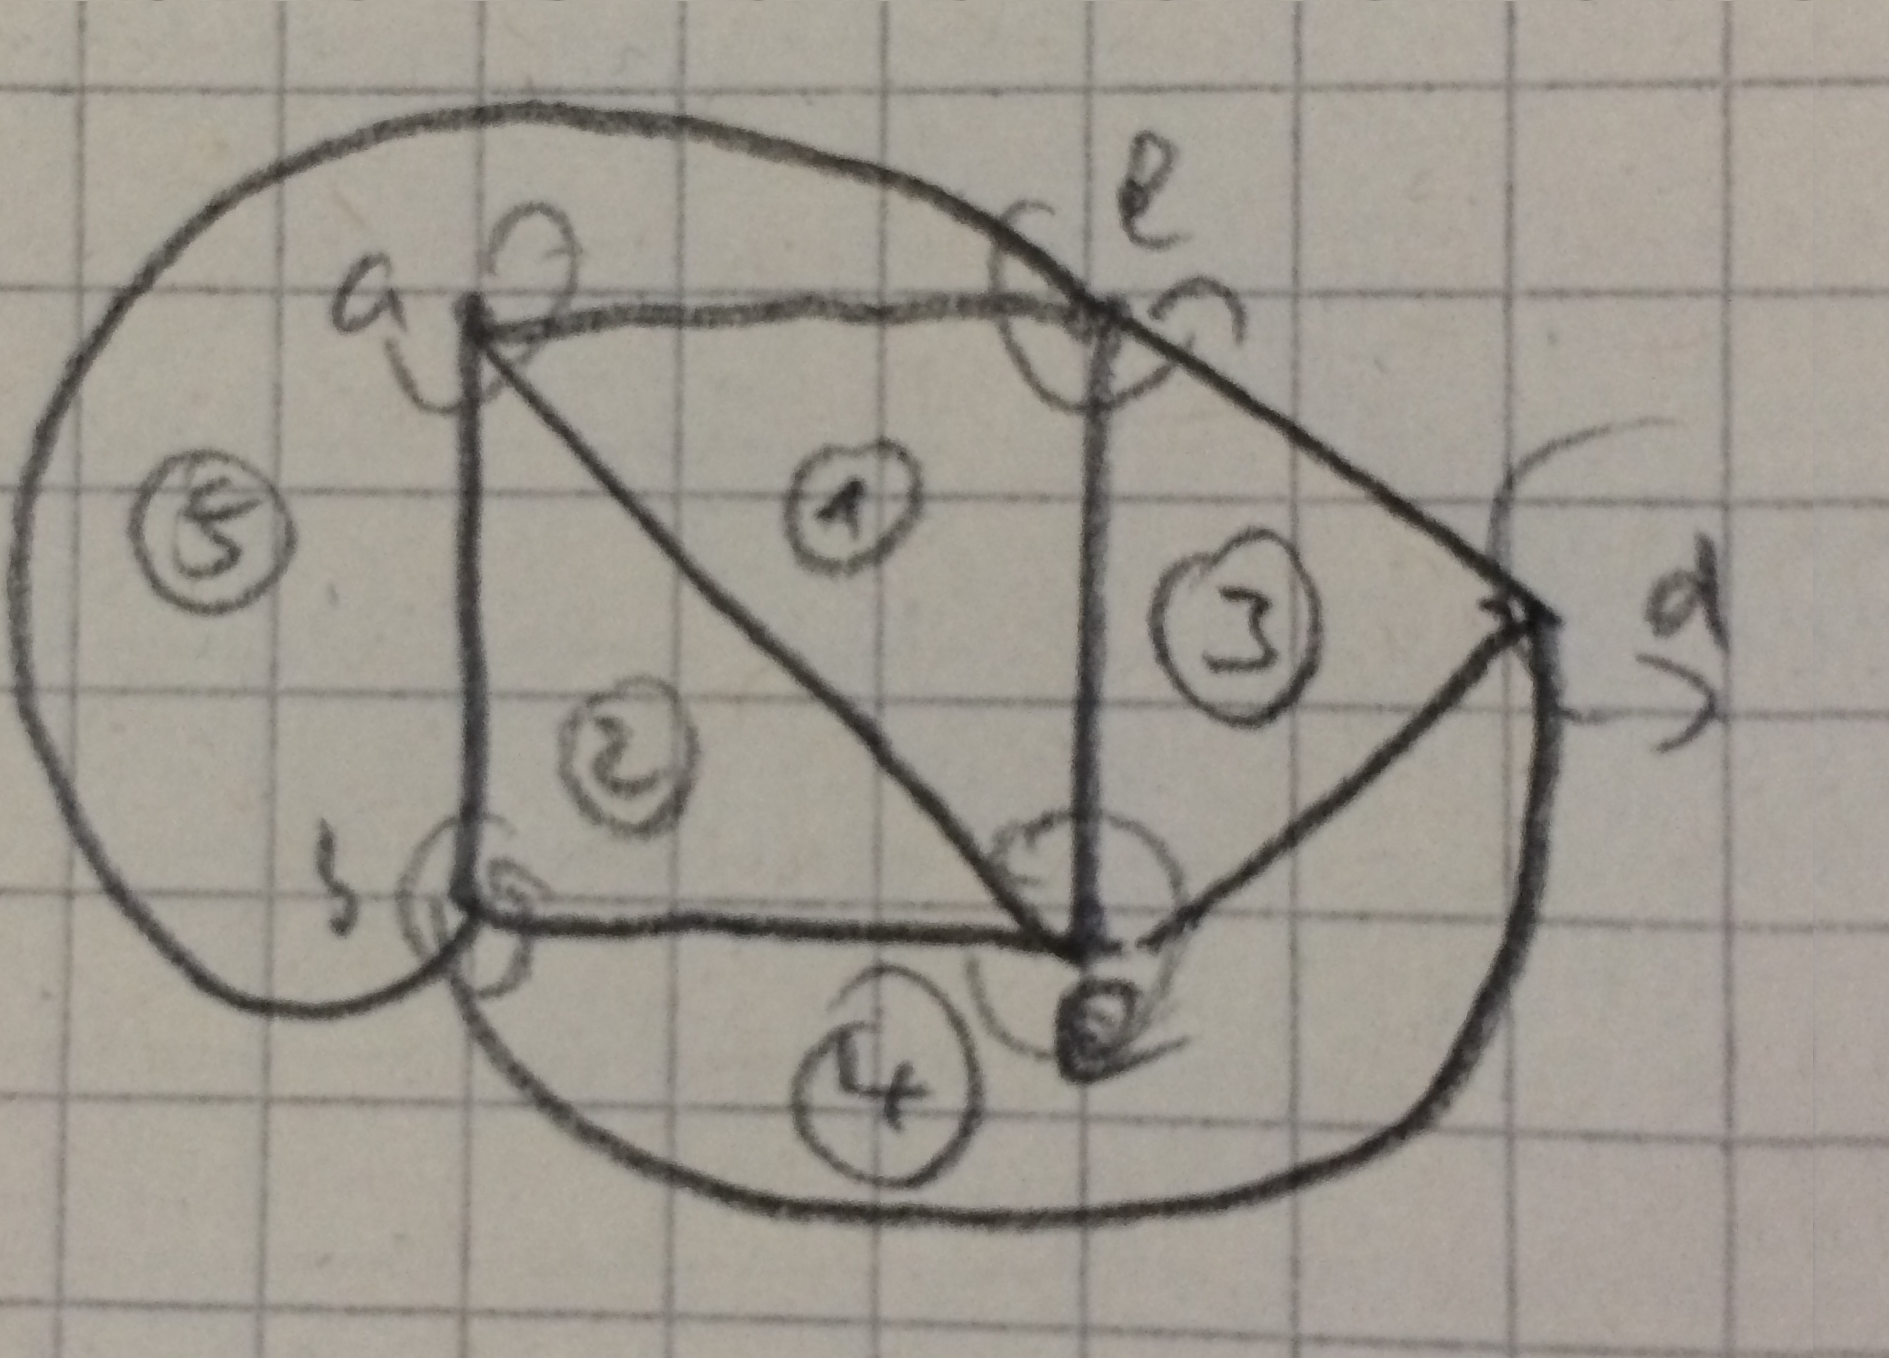
\includegraphics[scale=0.05]{12.png}\\
Eine planare Einbettung legt die Flächen fest, in jeder entpsrechenden Zeichnung.\\
Hier: 6 Flächen (Angegeben durch Knotenzyklus: ace, ace,cde,bdc,eba,bed\\
Flächendarstellung und Kantenlisten sind äquivalent (Adjazenzliste $\Leftrightarrow$ Fläche)\\
Im Allgemeinen existieren verschiedene planare Einbettungen für einen planaren Graphen G\\
Planare Einbettung ist eindeutig, falls G 3-Fach zusammenhängend\\
Euler Formel: Sei G eine zusammenhängende planare Einbettung mit n Knoten, m Kanten und f Faces, dann gilt: $n-m+f=2$\\
Beweis: Induktion über m\\
m=0: $n=1, f=1 $ ok\\
m=1: $n=2, f=1 $ ok\\
$m\geq 2$ IA: Für jede planare Einbettung mit weniger als m Kanten gilt die Formel. Sei nun G eine planare Einbettung mit m Kanten n Knoten und f Faces.\\
Fall1: G ist Baum d.h. azyklisch: $f=1$ Dann besitzt G einen Knoten v mit degree(v)=1 (Blatt)\\
Planare Einbettung $G\setminus \{v\}$ ist zusammenhängend und hat n-1 Knoten, m-1 Kanten und f=1 Faces\\
Fall2: G ist kein Baum -> $f>1$. Betrachte eine Kante e auf dem Zyklus. Betrachte die planare Einbettung $F\setminus\{e\}$ mit $m-1$ Kanten, n Knoten und $f-1$ Faces. $n-(m-1)+(f-1)=2$\\
Folgerung: Für jeden planaren Graph gilt $m\leq 3n -6$\\

Übung:\\
9.1: Kürzeste Wege in ayzklischen Graphen. Perfekte Wahl: Knoten aus U mit kleinster topologischer Nummer.\\
1. Idee: Berechne topologiesche Sortierung. Verwende PQ für U -> \oh{n*log(n)+m}\\
Besser: Kombination Topsort + kürzeste Pfade
\begin{lstlisting}[escapechar=!]
forall !$v\in V$! do
	INDEG[v] = indeg(v)
	if INDEG[v] == 0 then
		ZERO = ZERO !$\cup $! {v}
	fi
	DIST[v] = !$\infty$!
od
DIST[s] = 0
while ZERO !$\neq \emptyset$! do
	u = bel. Knoten aus ZERO
	ZERO = ZERO !$\setminus $!{u}
	forall !$v\in V$! mit !$(u,v) \in E$! do
		if --INDEG[v] == 0 then
			ZERO = ZERO !$\cup $!{v}
		fi
		d = DIST[u] + c(u,v)
		if d < DIST[v] then
			DIST[v] = d
		fi
	od
od
\end{lstlisting}
\oh{n+m}\\
9.2: pred-Verweise\\
Bellman/Ford + Algorithmus:\\
Falls count[v] > n: Durchlaufe die Pred-Verweise, starte in v. Markiere alle besuchten Knoten. Sobald wir auf bereits markierten treffen -> negativer Kreis\\
9.3/9.4: Negative Kosten bei Dijkstra\\
\hspace*{1cm}\\
\textbf{Euler Formel:} Planare Einbettung $n-m+f=2$\\
Folgerung 1: Sei G ein planarer Graph mit n Knoten und m Kanten, dann gilt $m\leq 3n-6$ mit m=\oh{n} Kanten -> viele Graphenprobleme können effizient gelöst werden.\\
Beweis: G besitzt eine planare Einbettung mit n Knoten, m Kanten und f Faces.\\
Definition: Ein planarer Graph heißt maximal planar, wenn er durch hinzufügen einer beliebigen Kante nicht mehr planar ist.\\
Beobachtung: In jeder planaren Einbettung eines max. planaren Graphen sind alle Faces Dreiecke.\\
$\Rightarrow$ Jede Fläche besitzt genau 3 Kanten. jede Kante gehört zu genau 2 Flächen.\\
Daraus folgt: $3f=2m \Rightarrow f=\frac{2}{3}m$. Eingesetzt in Eulerformel: $n-m+\frac{2}{3}m=2 \Rightarrow m=3n-6$\\
Folgerung 2: Sei G ein bipartiter planarer Graph dann gilt: $m\leq 2n-4$\\
Beweis: bipolar -> $\exists$ kein Kreis ungerader länge.\\
$\Rightarrow$ kleinste Flächen in planarer Einbettung von bipartiten Graphen sind Vierecke. Damit bestehen maximal planare bipartite Graphen nur aus Vierecken. $\Rightarrow 4f=2m \Rightarrow f=\frac{1}{2}m \Rightarrow m=2n-4$\\
Folgerung 3: Jeder planarer Graph besitzt einen Knoten v mit deg(v)$\leq$ 5\\
Foglerung 4: $K_5$ ist nicht planar. Für $K_5$ gilt n=5, m=10. Ein planarer Graph mit 5 Knoten hat maximal 9 Kanten.\\
Folgerung 6: $K_{3,3}$ ist nicht planar. n=6,m=9. $\Rightarrow$ bipartiter planarer Graph mit 6 Knoten hat max 8 Kanten.\\

Definition: Eine Knotenfärbung eines Graphen G=(V,E) ist eine Abbildung $num: V\rightarrow\{1,..,k\}$ sodass für jede Kante $(v,w)\in E$ gilt $num(v)\neq num(w)$. D.h. die durch eine Kante verbundenen Knoten haben stets verschiedene Farben\\
Problem: Finde minimales k, sodass eine Knotenfärbung existiert.\\
Bei planaren Graphen ist k=4 (Vierfarben-Problem). Wir zeigen k=5, ist einfacher.

\end{document}